% Use the University of Michigan thesis class.
\documentclass[letterpaper,12pt,oneside]{report}
\RequirePackage{times}
\usepackage{rac}

\newcommand{\MYIF}{\textbf{if }}
\newcommand{\MYELSE}{\textbf{else }}
\newcommand{\MYRETURN}{\textbf{return }}
\newcommand{\AlgBox}[1]{{\framebox[1.2\width]{\textbf{#1}}}}

\usepackage{epsfig,xspace,xspace,color,multirow}
\usepackage{graphicx,amssymb,amsmath,endnotes}
\usepackage{array,colortbl,booktabs}
\usepackage{times}
\usepackage{subfigure}
\usepackage{algorithm}
\usepackage{algorithmic}
\usepackage{amsthm}
\usepackage{url}
\usepackage{hyperref}
\usepackage{breakurl}
\usepackage{wasysym, pifont}
\usepackage{listings}
\usepackage{color}

\definecolor{dkgreen}{rgb}{0,0.6,0}
\definecolor{gray}{rgb}{0.5,0.5,0.5}
\definecolor{mauve}{rgb}{0.58,0,0.82}

\lstset{frame=tb,
  language=Java,
  aboveskip=3mm,
  belowskip=3mm,
  showstringspaces=false,
  columns=flexible,
  basicstyle={\small\ttfamily},
  numbers=none,
  numberstyle=\tiny\color{gray},
  keywordstyle=\color{blue},
  commentstyle=\color{dkgreen},
  stringstyle=\color{mauve},
  breaklines=true,
  breakatwhitespace=true
  tabsize=3
}

\usepackage{setspace}    % Allows you to specify the line spacing
\doublespacing           % \onehalfspacing for 1.5 spacing, \doublespacing for 2.0 spacing.

\if 0
\def\UrlBreaks{\do\A\do\B\do\C\do\D\do\E\do\F\do\G\do\H\do\I\do\J
\do\K\do\L\do\M\do\N\do\O\do\P\do\Q\do\R\do\S\do\T\do\U\do\V
\do\W\do\X\do\Y\do\Z\do\[\do\\\do\]\do\^\do\_\do\`\do\a\do\b
\do\c\do\d\do\e\do\f\do\g\do\h\do\i\do\j\do\k\do\l\do\m\do\n
\do\o\do\p\do\q\do\r\do\s\do\t\do\u\do\v\do\w\do\x\do\y\do\z
\do\.\do\@\do\\\do\/\do\!\do\_\do\|\do\;\do\>\do\]\do\)\do\,
\do\?\do\'\do+\do\=\do\#}
\fi

\newcommand{\etc}{\emph{etc.}\xspace}
\newcommand{\ie}{\emph{i.e.,}\xspace}
\newcommand{\eg}{\emph{e.g.,}\xspace}
\newcommand{\etal}{\emph{et al.}\xspace}
\newcommand{\wrt}{\emph{w.r.t.}\xspace}
\newcommand{\comment}[1]{{\color{red}[\textsf{#1}]}}

\newcommand{\MR}[1]{\multirow{2}{*}{#1}}
\newcommand{\MC}[1]{\multicolumn{2}{|c|}{#1}}
\newcommand{\hd}[1]{\small{\textbf{\texttt{#1}}}\normalsize}
\newcommand{\hds}[1]{\small{\textbf{\texttt{#1}}}}
\newcommand{\hdf}[1]{\small{\textbf{\texttt{#1}}}\footnotesize}

\newcommand{\UMICH}{$\sf\small{UMICH}$\xspace}
\newcommand{\RC}{$\small{\textbf{\texttt{RRC\_CONNECTED}}}\normalsize$\xspace}
\newcommand{\RI}{$\small{\textbf{\texttt{RRC\_IDLE}}}\normalsize$\xspace}
\newcommand{\RCB}{${\textbf{\texttt{RRC\_CONNECTED}}}\normalsize$\xspace}
\newcommand{\RIB}{${\textbf{\texttt{RRC\_IDLE}}}\normalsize$\xspace}
\newcommand{\FT}{$\sf\small{4GTest}$\xspace}
\newcommand{\TT}{$\sf\small{3GTest}$\xspace}
\newcommand{\mobiperf}{$\sf\small{MobiPerf}$\xspace}
\newcommand{\WG}{$\sf\small{Website~G}$\xspace}
\newcommand{\WY}{$\sf\small{Website~Y}$\xspace}

\newcommand{\IGL}{\includegraphics[width=0.995\textwidth]}
\newcommand{\IG}{\includegraphics[width=0.818\textwidth]}
\newcommand{\IGML}{\includegraphics[width=0.618\textwidth]}
\newcommand{\IGM}{\includegraphics[width=0.49\textwidth]}

\newcommand{\nsection}[1]{\vspace{-0.0em}\section{#1}\vspace{-0.0em}}
\newcommand{\nsubsection}[1]{\vspace{-0.0em}\subsection{#1}\vspace{-0.0em}}
\newcommand{\nsubsubsection}[1]{\vspace{-0.0em}\subsubsection{#1}\vspace{-0.0em}}
\newcommand{\ncaption}[1]{\vspace{-0.0em}\caption{#1.}\vspace{-0.0em}}


\begin{document}

\titlepage{Performance and Power Characterization of 3G/4G Networks and Optimizations of Mobile Applications}
{Junxian Huang}
{Doctor of Philosophy}
{Computer Science and Engineering}{2013}
{Associate Professor Z. Morley Mao, Chair \\
Associate Professor Jason N. Flinn \\
Associate Professor Robert Dick \\
Technical Staff Subhabrata Sen, AT\&T Labs -- Research}

\copyrightpage{Junxian Huang}

\initializefrontsections

% Dedication
\dedicationpage{\emph{To my family.}}

% Acknowledgments
%\acknowledgments[6]{
\startacknowledgementspage

I became a graduate student in the University of Michigan in the fall of 2008. Five years have passed and I would like to thank many people during this long and unique Ph.D. journey in my life. The completion of this dissertation would not be possible without anyone of them.

First of all, I would like to sincerely thank my advisor, Professor Z. Morley Mao. I first met her when I was an intern in Microsoft Research Asia in 2007, wondering about my future, and she offered me much helpful advice for pursuing a Ph.D. degree in the U.S. Morley has provided me excellent and professional guidance on various research projects throughout my Ph.D. study, given her expertise in the computer networking and mobile computing, as well as delicious birthday cakes, when even I forgot my birthday myself. Moreover, she helped me gain the confidence, ability and most importantly, the enthusiasm to tackle difficult real-world problems. Her diligence and enthusiasm has set a great model for me and the experiences working with her would be my life-long treasure.

I am greatly thankful for my mentors Kun Tan and Yongguang Zhang in Microsoft Research Asia (Beijing 2007), Yinglian Xie and Fang Yu in Microsoft Research Silicon Valley (California 2010), Subhabrata Sen and Oliver Spatscheck in AT\&T Labs - Research (New Jersey 2012). I am fortunate to work with these knowledgeable and excellent researchers. I enjoyed my internships, which would be my unforgotten memories. I also enjoyed the conversations with them about exciting research ideas, and about career and life as well. Many of their words have kept ringing in my mind, helping me to improve.

I would like to express my deep gratitude to Professor Jason Flinn, Dr. Subhabrata Sen and Professor Robert Dick for serving as my thesis committees. Their valuable suggestions and comments have greatly helped me improve this dissertation. My grateful thanks are also due to Professor Scott Mahlke, Professor J. Alex Halderman for their excellent teaching on my core computer science courses, and Dr. Ming Zhang and Dr. Paramvir Bahl for their priceless help for me in writing and presenting the my first conference paper~\cite{mobisys.3gtest}.

It is hard for me to forget the great professors during my undergraduate study in Tsinghua University who taught me the basics in computer science and helped me find the joy in this area. Their names include Xiping Mao, Wei Chen, Hong Wang, Jianhua Feng, Zhongxin Xu (who passed away in 2010 and is long remembered), Shimin Hu, Ning Su, \etc I owe my special thanks to Professor Andrew Chi-Chih Yao, who included me in his first special pivot class, where I have received great education in computer science, and he himself also demonstrated what a great computer scientist and a Turing Award winner is like.

I would like to thank all my friends and colleagues at Michigan. I have worked closely with Dr Feng Qian and Qiang Xu since the first day of my Ph.D. study. Dr. Ying Zhang, Dr. Xu Chen and Dr. Zhiyun Qian are former members of our research group and they are also my good friends. I am grateful for my roommate Lujun Fang. My thanks also go to my other friends and colleagues in the Computer Science department at Michigan, including, but not limited to Bin Liu, Yunjing Xu, Yudong Gao, Birjodh Tiwana, Zhaoguang Wang, Lide Zhang, Mark Gordon, Caoxie Zhang, Fangjian Jin, Zhe Chen, Kee Shen Quah, Li Qian, Sanae Rosen, Bangxin Hu, Jie Yu, Xinyu Zhang, Timur Alperovich, Yihua Guo, Yuanyuan Zhou, Haokun Luo, Qi Chen. I am thankful for University of Michigan Table Tennis Club (UMTTC) and University of Michigan Chinese Drama Club for bringing me many good days and good friends: Weilun Xu, Hang Zhao, Allen Hung, Ason Chiang, Bo Bi, Yang Zhou, Tomas Fuentes-Afflick, Lang Ming, Yuhua Wang, Beimin Zhu, \etc I want to thank my piano teachers Alexandra Lynelle James, Yuanchang Zhou, Shuai Wang, and my table tennis coaches David Kleshchik, Naihui Liu, Qing Miao for helping me fulfill my childhood dreams. I would also like to thank my other friends outside Michigan for appearing in and shaping my life: Jianfeng Gao, Qi Xie, Wentao Han, Jingyue Wu, Hui Min, Ruizhe Li, Chengwei Guo, Yifang Yuan, Jiajie Zhu, Haohui Mai, Yini Xu, Ning Ding, Shan Zhou, Zhaojie Cheng, Dongdong Peng, Simin Zhang, Tian Guo, Yi Chen, Di Zhang, Zhenqiang Gong, \etc

I could not love University of Michigan more. ``For today, Goodbye; For tomorrow, Good Luck; Forever, GO BLUE!'' I will remember Ann Arbor, the most beautiful town in the world. I will miss Mr. CSE raccoon, Mr. North-Campus turkey, unnamed geese and deer, and I will be a fighting wolverine wherever I go!

Finally, I would like to express my deepest thanks to my beloved parents, Xuemeng Huang and Zhaoxia Wang, and my dearest grandparents Shu Huang, Lingzhi Liu, Shengqin Wang (who passed away in 2008 to my greatest sadness) and Xiuhua Ma for their enduring love, support and encouragement throughout my life. This dissertation is dedicated to them.

\label{ACKNOWLEDGEMENTS}


\tableofcontents     % Required
\listoftables        % Required if there is more than one table
\listoffigures       % Required if there is more than one figure
\listofappendices

\startabstractpage
{Performance and Power Characterization of Cellular Networks and Mobile Application Optimizations}
{Junxian Huang}{Chair: Z. Morley Mao}

Smartphones with cellular data access have become increasingly popular with the wide variety of mobile applications. However, the performance and power footprint of these mobile applications are not well-understood, and due to the unawareness of the cellular specific characteristics, many of these applications are causing inefficient radio resource and device energy usage. In this dissertation, we aim at providing a suite of systematic methodology and tools to better understand the performance and power characteristics of cellular networks (3G and the new LTE 4G networks) and the mobile applications relying upon, and to optimize the mobile application design based on this understanding.

We have built the \mobiperf tool to understand the characteristics of cellular networks. With this knowledge, we make detailed analysis on smartphone application performance via controlled experiments and via a large-scale data set from one major U.S. cellular carrier. To understand the power footprint of mobile applications, we have derived comprehensive power models for different network types and characterize radio energy usage of various smartphone applications via both controlled experiments and 7-month-long traces collected from 20 real users. Specifically, we characterize the radio and energy impact of the network traffic generated when the phone screen is off and propose the screen-aware traffic optimization. In addition to shedding light to the mobile application design throughout our characterization analysis, we further design and implement a real optimization system \NAMEFULL, which uses historical traffic features to make predictions and intelligently deallocate radio resource for improved radio and energy efficiency.


\oldstuff{

keywords:
Cellular Networks
Network Characterization
Smartphone Energy Model
LTE Networks
Mobile Application Optimization
TCP in Cellular Networks


some suggestions from Morley:

Combine I and II.  (II is very short).
The thesis statement in I is not quite concise and clear enough.
It needs to be a single sentence that captures problem statement and your solution/approach.
The texts starting with "However..." are too long.

I haven't the texts in detail, but it appears that there is very little transition across chapters.

The results in III and IV are a little dated, please clearly mark when these experiments were done.
(Please do so for the other results as well in other chapters.)



The transition between chapters is quite weak and it should refer back to the
thesis statement. 

There are five technical chapters of completed work, which is quite extensive, but not as coherent as it could be.  One way to make the dissertation easier to navigate is to provide a more clear roadmap in chapter 1, which currently summarizes each technical chapter.  It would be useful to broadly characterize these five pieces into:
1. mobile network characterization  (performance and RRC models)
2. mobile application characterization (protocol interaction)
    interplay between mobile app and network: energy implications
3. optimization to improve performance and energy.

By referring back to these three aspects, each of the five technical pieces can fit together better in the dissertation.

Chapter IX is written as if the author plans to continue to do some of the work.
It may be more appropriate to clarify the remaining challenges for others who are interested in following up on these topics.  It needs to clearly outline how these challenges may change as smartphones become more powerful, networks become faster and more energy efficient, and applications behavior also evolves.



Comments from Morley after defense

+ Add table of roadmap of results in intro so that it does not look like data dump.
+ What are the long term conclusions for cellular networks and what may change?

Please also take these comments into considerations besides the ones I gave you.

How persistent are some of the observations as networks and phones and applications evolve?  (maybe you want to emphasize the measurement methodology besides the measurement findings).

How are these observations different from Internet observations?

RadioProphet:  explain the principles more clearly.  need better comparison.
Idle time prediction is an old problem, how is it different from previous work?
What are the insights observed?
(During the defense, you seem to indicate that per application based prediction will not work, I agree with you, but per-application based prediction probably will be more accurate?  can you confirm that?

Slide 67: you need to also show the bad result: how much worse is your saving than FD).
Need to compare with less agressive FD (what is the common FD setting on today's phones?)

Introduction:
Needs to have a roadmap of different measurement results in all the chapters: when they are collected, what are the main findings.
Need to have a summary of the findings, key contributions, highlights of the important lessons learned.

}

\label{Abstract}


\startthechapters
\chapter{Introduction}
\label{chap:intro}

Smartphones with cellular data access have become increasingly popular across the globe, with the wide deployment of 3G and emerging LTE~\cite{3gpp.lte} networks, and a plethora of applications of all kinds. In the third quarter of 2009, the global smartphone shipments reached 41.4 million units~\cite{smartphoneStat}. As of the third quarter of 2012, the global smartphone shipments reached 173.7 million~\cite{smartphoneStat2} with 61.3\% year-on-year increase in average. It is expected that in the next few years smartphone sales will continue to grow.  Vendors, such as Samsung, Apple, and HTC offer a variety of smartphones equipped with increasingly faster CPUs and larger memory, though still lagging behind desktop or laptop systems. With access to various high-speed 3G networks, such as EVDO and UMTS, and the LTE 4G networks, they are powerful enough to run modern operating systems and sophisticated network applications such as web browsing, email, and streaming media. 

Unlike traditional Internet-based applications, whose performance is mostly constrained by the wired network, network application performance on smartphones with limited physical resources also heavily depends on factors including hardware and software on the phone as well as the quality and load of wireless link. Understanding the application performance on smartphones is important for the purpose of assisting consumers in choosing carriers and phones and guiding application developers in designing intelligent software. Moreover, cellular network operators and smartphone hardware and software vendors can use this knowledge to optimize networks and phones for better end-user experiences. Similarly, content providers can leverage this knowledge to better customize content for mobile users. However, this task is quite challenging since the performance of network applications on smartphones is poorly understood thus far, due to a lack of a systematic approach for controlled experiments and comparative analysis, and especially because the network performance of the underlying cellular networks is not well understood. In this thesis, we take one of the first steps to thoroughly study the performance of cellular networks and smartphone applications.

In addition to network performance aspect, we also study the energy footprint for smartphone applications. Today�s cellular systems operate under diverse resource constraints: limited frequency spectrum, network processing capability, and handset battery life. Optimizing energy footprint for smartphone applications is important for end-users. In the meanwhile, optimizing the radio resource usage is of great interest for mobile operators to minimize cost and guarantee quality of service.


\nsection{Characterizing Cellular Network Performance} Since 2008, We have been working on devising systematical methodologies and developing tools for characterizing cellular network performance directly from end users. The tools developed includes \TT~\cite{3gtest}, \FT~\cite{4gtest} and \emph{MobiPerf}~\cite{mobiperf}~\footnote{Notably, \emph{MobiPerf} has received both the \emph{Open Internet App Award} and the \emph{People's Choice App Award} in the \emph{FCC Open Internet Apps Challenge}~\cite{fcc.award}. It is now an open-source project~\cite{mobiperf.repo} that we are actively working on and this project is in joint collaboration among University of Michigan, M-Lab~\cite{mlab} and University of Washington.}, which have cumulatively over 150,000 users from over 190 countries or regions. In these measurement tools, we have devised methods to accurately measure round-trip time (RTT), DNS lookup time, uplink/downlink bandwidth, loss rate, and other network performance metrics for 3G, WiMAX and LTE 4G networks and compare those with WiFi networks.

Our study is among one of the first studies of the network characteristics of commercial LTE networks. Initiated in 2004 by {\em 3rd Generation Partnership Project} (3GPP),  the {\em Long Term Evolution} (LTE), commonly referred to as a type of 4G wireless service, aims at enhancing the {\em Universal Terrestrial Radio Access Network} (UTRAN)  and optimizing radio access architecture~\cite{3gpp.lte}. Since 2009, LTE starts entering the commercial markets and is available now in more than 10 countries, with an expectedly fast-growing user base. The targeted user throughput is 100Mbps for downlink and 50Mbps for uplink, significantly higher than the existing 3G networks, with less than 5ms user-plane latency~\cite{tr25.913}. Understanding the actual user-perceived network performance for LTE network and how it compares with its predecessor 3G and its competitors, \eg WiFi and WiMAX, is important, yet not straightforward. Our forementioned tool \FT, with enhanced measurement design and global server support, allows us to characterize network performance of LTE and other mobile networks~\cite{huang_mobisys12}.


\nsection{Anatomizing Smartphone Application Performance}
In order to understand the key factors that affect smartphone application performance, we develop a systematic methodology for comparing this performance along several key dimensions such as carrier networks, device capabilities, and server configurations~\cite{mobisys.3gtest}. We perform detailed analysis to help carriers, phone vendors, content providers, and application developers gain insight. For example, for carriers, we infer various network level problems, \eg high latency or high loss rate, which they can directly take action on. For phone vendors, we identify performance bottlenecks on the devices or issues associated with the content. These issues can be resolved either independently or by cooperating with content providers. And for application developers, we evaluate factors such as the overhead of HTML rendering and Javascript execution given a particular software configuration. 

%anatomize app performance
Compared with 3G, LTE significantly improves the network performance. Meanwhile, device processing capability and software design have also improved remarkably over the last two years~\cite{mobisys.3gtest}. To understand the potential performance bottleneck shift for smartphone applications, we perform longitudinal case studies of several popular applications on Android, especially for web browsing applications. With the help of CPU, network and power traces, we compare the determinant factors on smartphone applications in 2009~\cite{mobisys.3gtest} and in 2011~\cite{huang_mobisys12}. We identify that the performance bottleneck for web-based applications lies more in the device�s processing power than in the network for the LTE networks.

\nsection{Studying Effect of Network Protocol and Application Behavior on Performance for LTE Networks}
Despite it fast increasing user base, the interplay between mobile applications, protocol and the network for the commercial LTE networks still remain unexplored. We thoroughly study these topics of the LTE network with a data set covering around 300,000 real LTE users in a large metropolitan area for 10 days. We revisit basic network metrics in the LTE network and compare with previously studied network conditions. We also observe that a high downstream queueing delay, likely due to bufferbloat,  has caused TCP congestion window collapse upon one packet loss. With the help of TCP Timestamps option, we have devised a lightweight passive bandwidth estimation algorithm, allowing us to observe that for 71.26\% of the large flows, the bandwidth utilization ratio is below 50\%. We find that TCP may not fully utilize the fast-varying available bandwidth when RTT is large in the LTE network. Upon further analysis, we identify 52.61\% of all downlink TCP flows have been throttled by TCP receive window and data transfer patterns for some popular applications are both energy and network unfriendly.

\nsection{Understanding Power Characteristics of 4G LTE Networks}
Besides higher bit rate, lower latency and many other service offerings for LTE, {\em user equipment} (UE) power saving is an important issue and there has been increasing interest in understanding the power characteristics of LTE networks, compared with 3G/WiFi networks. LTE employs {\em Orthogonal Frequency Division Multiplex} (OFDM~\cite{ts36.211}) technology, which suffers from poor power efficiency. To save power, LTE uplink uses an special implementation of OFDM called SC-FDMA for uplink, with improved power efficiency. {\em Discontinuous reception} (DRX) has been employed by existing wireless mobile networks to reduce UE energy consumption. In UMTS~\cite{ts25.304}, during the idle state, UE periodically wakes up to check paging messages and sleeps for the remaining time. LTE supports DRX for both \RC and \RI modes~\cite{ts36.321}, seeking more opportunities to conserve UE battery. DRX is configured at a per-UE basis and its configuration incurs tradeoff among UE power saving, channel scheduling delay, and signaling overhead.

To understand this tradeoff, existing studies use either total DRX-on time to estimate UE power usage~\cite{vtc.drx, ieee.drx}, or a simplified LTE power model~\cite{iswcs.lte, icc.drx}, which ignores the impact of downlink/uplink data rates. In this paper, we develop the first empirically derived comprehensive power model of a commercial LTE network, which accurately models UE energy usage with less than 6\% error rate. Also, existing studies~\cite{vtc.drx, ieee.drx, iswcs.lte, icc.drx} heavily rely on synthetic packet models instead of real user traces. Our study is the first that leverages a comprehensive real user data set, we call \UMICH, consisting of 5-month traces of 20 smartphone users, to analyze the impact of LTE parameter configuration on realistic application usage patterns. We carefully investigate the energy usage in 3G, LTE, and WiFi networks and evaluate the impact of configuring LTE-related parameters. Despite several new power saving improvements, we find that LTE is as much as 23 times less power efficient compared with WiFi, and even less power efficient than 3G, based on the user traces and the long high power tail is found to be a key contributor.

\nsection{Optimizing Energy Usage in Cellular Networks}
With the knowledge of performance and power characteristics of 3G/4G cellular networks, we study how we can optimize the resource (radio and energy) utilization of smartphone applications. Cellular networks are typically characterized by limited radio resources and significant device power consumption for network communications. The battery capacity of smartphones cannot be easily improved due to physical constraints in size and weight. Hence, battery life remains a key determinant of end-user experience. Given the limited radio resources in these networks and device battery capacity constraints, optimizing the usage of these resources is critical for cellular carriers and application developers. Achieving such energy efficiency for mobile devices when connected to cellular networks without incurring excessive network signaling overhead, even despite diverse application and user behavior, still remains a rather difficult and yet important challenge to tackle. Energy use due to network access, particularly cellular networks, is becoming increasingly dominant due to numerous network-based smartphone applications. In many cases, achieving network energy savings must reside on the mobile device's OS to effectively and centrally manage the data scheduling decisions transparent to applications and with minimal changes to the network.

The key mechanism that determines the energy consumed by cellular network interface is the radio resource control (RRC) state machine~\cite{imc.3g} pre-defined by carriers (covered in more details in Section~\ref{sec:bkg.rrc}) that governs when radio resources are acquired and released. Previous studies~\cite{imc.tailender, imc.3g, qian10_icnp, huang_mobisys12} have shown that the origins of low resource efficiency comes from the way radio resources are \emph{released}. Radio resources are only released after an idle time (\aka Radio Resource Control (RRC) tail~\cite{imc.tailender}) controlled by a statically configured inactivity timer. The tail is necessary and important for cellular networks to prevent frequent state promotions (resource allocation), which can cause unacceptably long delays for the UE, as well as additional processing overheads for the radio access network~\cite{poor, infocom_lee}. During the tail time, radio energy is essentially wasted. Values as large as 11.6 seconds are configured~\cite{huang_mobisys12} in current networks, contributing to about half of the total radio energy on user handsets (UEs) spent in idle times for common usage scenarios.

Without knowing when network traffic will occur, large tail timer settings are essentially a conservative way to ensure low signaling overhead due to state transitions, as signaling is known to be a bottleneck for cellular networks.  Furthermore, they also help minimize performance impact experienced by users caused by state promotion delays incurred whenever radio resource is acquired.
Given that application and user behavior are not random, using a statically configured inactivity timer is clearly suboptimal. Smaller static timer values would help reduce radio energy, but is not an option due to the risk of overloading cellular networks caused by signaling load increase.

An attractive alternative is to configure the timer dynamically --- adaptively performing radio resource release either signaled by the UE or triggered by the network itself by monitoring the UE traffic, accommodating different traffic patterns, improving the overall resource efficiency. But the key challenge is determining \emph{when} to release resources, which essentially comes down to accurate and efficient prediction of the idle time period. Clearly, the best time to do so is when the UE is about to experience a long idle time period, otherwise the incurred resource allocation overhead (\ie signaling load) is wasteful due to unnecessary radio state transitions, and the achieved resource savings are very small. Therefore, accurate and efficient prediction of the idle time period is a critical prerequisite for dynamic timer schemes.

We propose \NAMEFULL (\NAME), a practical system that makes dynamic decisions to deallocate radio resources based on accurate and efficient prediction of network idle times. Using 7-month-long real-world cellular traces, we comprehensively evaluate it using various traffic features and machine learning algorithms. Properly configured, it correctly predicts 85.88\% of idle time instances, achieving radio energy savings of 59.07\%, at the cost of 91.01\% of additional signaling overhead, significantly outperforming existing proposals. It incurs negligible energy overhead and has fast response times, demonstrating the practicality of deploying the system on contemporary smartphones.

Besides, we also consider a novel angle to the above problem orthogonal to \NAME and explore the impact of {\bf screen status}, \ie whether the screen is on or off, on the device's network traffic patterns. We find that off-screen traffic accounts for 58.5\% of the total radio energy consumption although their traffic volume contribution is much smaller. Such unexpected results are attributed to the unique cellular resource management policy that is not well understood by developers, leading to cellular unfriendly mobile apps. We then make a further step by proposing screen-aware optimization, given that the screen status is easy to monitor for most mobile OSes. We propose that the screen-off traffic should not be treated the same as the screen-on traffic for traffic optimization purposes, and the former can be optimized more aggressively.  The main intuition is that the user (and possibly application)  behavior have significant differences when the screen is on {\em v.s.} off, resulting in different traffic patterns and different performance requirements. When the screen is off, there is a much higher chance that the user is not actively interacting with the device and the network traffic is most likely to be more delay tolerant. Hence we can be more aggressive in optimizing this traffic using techniques such as batching and fast dormancy. In contrast, when the screen is on, it is harder to predict the delay sensitivity of the network traffic and aggressive optimizations may harm the user experience. To validate this intuition, we characterize the screen-off traffic for a real-world user data set and evaluate the benefits of using ``screen-aware'' optimization for balancing UE energy savings and the resulting overheads in radio resource usage and response delay. The proposed screen-aware optimization focuses on the overall device traffic, and is complementary to other efficiency improvement efforts, \eg better application design. Our proposal can better balance the key tradeoffs in cellular networks. 






\section{Thesis Organization}

This dissertation is structured as follows. Chapter~\ref{chap:bkg} provides necessary backgrounds for resource management in cellular networks. We present the design of \mobiperf tool and network performance characterization in Chapter~\ref{chap:net} followed by the smartphone application performance study in Chapter~\ref{chap:app}. We study the effect of network protocol and application behavior on performance for one large commercial LTE Network in Chapter~\ref{chap:tcp}.  We analyze the power characterization of smartphone applications in Chapter~\ref{chap:power} and present the design, implementation and evaluation for the smartphone energy optimization system \NAME in Chapter~\ref{chap:optimize}. We summarize the related works in Chapter~\ref{chap:related}, before concluding in Chapter~\ref{chap:conc}.




\oldstuff{
Chapter~\ref{chap:net}: MobiPerf: 3G/4G network performance characterization
	+ Motivation
	+ Metrics
	+ Design and implementation of tools
	+ Results
	+ Implications (compare across network types, compare over time)
	
Chapter~\ref{chap:app}: smartphone application study
	+ Motivation
	+ Web based application running time breakdown.
	+ Video/audio streaming applications (sigcomm submission, mobisys10)
	
Chapter~\ref{chap:tcp}: LTE traffic pattern study Interplay of TCP, smartphone applications and cellular networks
	+ Motivation
	+ Sigcomm draft characterization part
	+ Sigcomm draft inefficient TCP part
	
Chapter~\ref{chap:power}: smartphone power model
	+ Motivation
	+ Measurement methodology: tools, experiments
	+ Power model
	+ How to use power model: trace-driven network/power simulation methodology (validation)
	+ Screen status's impact on traffic pattern
	+ Power footprint of apps (mobisys12)
		
Chapter~\ref{chap:optimize}: RadioProphet: optimize for better balance of performance and energy
	+ RadioProphet
	+ screen-aware optimization

Chapter~\ref{chap:related}: related work
}

\chapter{Background} \label{chap:bkg}

This section provides sufficient background on resource management in cellular networks, especially for the LTE networks.

\nsection{Radio Resource Control (RRC) State Machine}
\label{sec:bkg.rrc}

\begin{figure}[t]
\centering
\IG{figures/rp/rrc.eps}\\
\ncaption{\small{RRC State Machine of (a) a large 3G UMTS carrier in the U.S., and (b) a large 4G LTE carrier in the U.S. The radio power consumption was measured by a power monitor on (a) an HTC TyTn II smartphone, (b) an HTC ThunderBolt smartphone}}
\label{fig:rrc}
\end{figure}

To efficiently utilize the limited resources, cellular networks employ a resource management policy distinguishing them from wired and Wi-Fi networks. In particular, there is a radio resource control (RRC) state machine~\cite{imc.3g} that determines radio resource usage based on application traffic patterns, affecting device energy consumption and user experience. Similar RRC state machines exist in different types of cellular networks such as UMTS~\cite{imc.3g}, EvDO~\cite{ChatterjeeD02} and 4G LTE networks~\cite{huang_mobisys12}, although the detailed state transition models may differ.

\textbf{RRC States.} In 3G UMTS networks, there are usually three RRC states~\cite{imc.3g, mobisys.aro}. \RI is the default state when the UE is turned on, with no radio resource allocated. \RD is the high-power state enabling high-speed data transmission. \RF is the low-power state in between allowing only low-speed data transmission. In 4G LTE networks, the low-power state is eliminated due to its extremely low bandwidth (less than 20 kbps) so there are only two RRC states named \RC and \RI~\cite{tr25.813, ts36.331}.

\textbf{State Transitions.}
As shown in Figure~\ref{fig:rrc}, regardless of the specific state transition model, there are two types of state transitions. State promotions switch from a low-power state to a high-power state. They are triggered by user data transmission in either direction. State demotions go in the reverse direction, triggered by inactivity timers configured by the radio access network (RAN). For example, as shown in Figure~\ref{fig:rrc}b, at the \RC state, the RAN resets the \RC$\rightarrow$ \RI timer to a constant threshold $T_{tail}$=11.6 seconds whenever it observes any data frame. If there is no user data transmission for $T_{tail}$ seconds, the \RC$\rightarrow$ \RI timer expires and the state is demoted to \RI. The two timers in 3G UMTS networks use similar schemes (Figure~\ref{fig:rrc}a).

State promotions and demotions incur \emph{promotion delays} and \emph{tail times}, respectively, which distinguish cellular networks from other types of access networks.

\textbf{State promotions} incur a long ``ramp-up'' delay of up to several seconds during which tens of control messages are exchanged between the UE and the radio access network (RAN) for resource allocation. Excessive state promotions increase the signaling overhead at the RAN and degrade user experience, especially for short data transfers~\cite{3gpp:090941, qian10_icnp}.

\textbf{State demotions} incur \emph{tail times} that cause waste of radio resources and the UE energy~\cite{imc.tailender, imc.3g}. A tail is the idle time period matching the inactivity timer value before a state demotion, \eg the tail time is 11.6 seconds in Figure~\ref{fig:rrc}b. During the tail time, the UE still occupies transmission channels, and its radio power consumption is kept at the corresponding level of the RRC state.
As an example of the negative impact of the tail effect, periodically transferring small data bursts (\eg every one minute) can be extremely resource-inefficient in cellular networks due to the long tail appended to each periodic transfer instance which is small in size and short in duration~\cite{qian12_www}.

%A recent study~\cite{qian12_www} shows that for popular smartphone applications such as Facebook and Pandora, periodic transfers account for only 1.7\% of the overall traffic volume but contribute to 30\% of the total UE radio energy consumption.

\textbf{Adaptive Release of Radio Resources.} Why are tail times necessary? First, the overhead of resource allocation (\ie state promotions) is high and tail times prevent frequent allocation and deallocation of radio resources. Second, the current radio resource network has no easy way of predicting the network idle time of the UE, so it conservatively appends a tail to every network usage period. This naturally gives rise to the idea of letting the UE actively request for resource release: once an imminent long idle time period is predicted, the UE can actively notify the RAN to immediately perform a state demotion. Based on this intuition, a feature called fast dormancy has been proposed
to be included in 3GPP Release 7~\cite{fast.dormancy.1} and Release 8~\cite{fast.dormancy.2}. It allows the UE to send a control message to the RAN to immediately demote the RRC state to \RI (or a hibernating state called \RPCH) without experiencing the tail time. Fast dormancy is currently supported by several handsets~\cite{fast.dormancy.2}, which can dramatically reduce the radio resource and the UE energy usage while the potential penalty is the increased signaling load when used aggressively~\cite{3gpp:090941, qian10_icnp}. In this work we propose robust methodology for predicting the idle time period, enabling more effective usage of fast dormancy.



\nsection{RRC and Discontinuous Reception (DRX) in LTE}
\label{sec:bkg.lte}

In this section, we provide more details for RRC in LTE in addition to Section~\ref{sec:bkg.rrc}, as well as Discontinuous Reception (DRX) mechanisms in LTE.
\begin{table*}[t]
\centering
\small
\begin{tabular}{|c|c|c|c|}\hline
Symbol & Full name & Measured value & Description \\\hline\hline
\MR{$T_i$} & \MR{DRX inactivity timer} & \MR{100ms} & UE stays in Continuous Reception \\
 & & & for $T_i$ before DRX starts when idling \\\hline
\MR{$T_{is}$} & \MR{Short DRX cycle timer} & \MR{20ms} & UE remains in Short DRX for $T_{is}$ \\
 & & & before entering Long DRX when idling \\\hline
\MR{$T_{tail}$} & \MR{RRC inactivity timer} & \MR{11.576s} & UE stays in RRC\_CONNECTED~for  \\
  & & & $T_{tail}$ before demoting to RRC\_IDLE\\\hline
\MR{$T_{on}$} & RRC\_CONNECTED & \MR{1ms} & The on duration of UE during each \\
  & On Duration timer & &  DRX cycle in RRC\_CONNECTED \\\hline
\MR{$T_{oni}$} & RRC\_IDLE & \MR{43ms} & The on duration of UE during \\
  & On Duration timer & & each DRX cycle in RRC\_IDLE \\\hline
\MR{$T_{ps}$} & \MR{Short DRX cycle} & \MR{20ms} &The cycle period of Short DRX \\
  & & & in RRC\_CONNECTED\\\hline
\MR{$T_{pl}$} & \MR{Long DRX cycle} & \MR{40ms} & The cycle period of Long DRX \\
  & & & in RRC\_CONNECTED \\\hline
\MR{$T_{pi}$} & \MR{RRC\_IDLE~DRX cycle} & \MR{1.28s} & The cycle period of DRX \\
  & & & in RRC\_IDLE \\\hline
\end{tabular}
\ncaption{Important LTE RRC and DRX parameters}
\label{tab:parameter}
\end{table*}

\begin{figure}[t]
\centering
\IG{figures/mobisys12/sm.eps} \\
\ncaption{RRC state transitions in LTE network}
\label{fig:sm}
\end{figure}

As shown in Figure~\ref{fig:sm}, at \RC~state, UE can be in one of the three modes: Continuous Reception, Short DRX, and Long DRX. While at \RI~state, UE is only in DRX mode. Table~\ref{tab:parameter} enumerates a list of important LTE parameters, which have significant impact on UE's radio energy consumption, user experience, and signaling overhead for cell towers. The terms in Table~\ref{tab:parameter} are used consistently throughout this paper.

If UE is initially in \RI~state and receives/sends one packet, regardless of the packet size, a state promotion from \RI~to \RC occurs with a relatively stable delay, similar to the promotion from IDLE to DCH/FACH in UTMS network~\cite{imc.3g}. We define the LTE promotion delay to be $T_{pro}$\footnote{$T_{pro}$ is a measured system property, different from the configurable LTE parameters in Table~\ref{tab:parameter}.} consistently throughout this paper. During this period, radio resources are allocated to the UE.  

After being promoted to \RC, UE enters Continuous Reception by default and keeps monitoring the {\em Physical Downlink Control Channel} (PDCCH), which delivers control messages to UE. UE also starts the DRX inactivity timer $T_i$, which is reset every time UE receives/sends a packet. Upon $T_i$'s expiration without seeing any data activity, UE enters the Short DRX mode.

\begin{figure}[t]
\centering
\IG{figures/mobisys12/drx.eps} \\
\ncaption{Illustration of the LTE DRX in \RC}
\label{fig:drx}
\end{figure}

Discontinuous Reception (DRX)~\cite{ts36.321, 4gbook}, illustrated in Figure~\ref{fig:drx}, is adopted by LTE for UE to ``micro-sleep'' to reduce power consumption while providing high QoS and connectivity. DRX in \RC and \RI have similar mechanisms, but different parameter settings. A DRX cycle includes an On Duration during which the UE monitors PDCCH. UE rests for the rest of the cycle to save energy. The tradeoff between battery saving and latency is the guideline for determining the parameterization of DRX cycle. With a fixed On Duration, a longer DRX cycle reduces energy consumption of UE while increasing user-perceived delay, and a shorter DRX cycle reduces the data response delay at the cost of more energy consumption. Short DRX and Long DRX modes, having the same On Duration and differing in cycle length, are to meet these conflicting requirements.

When UE enters Short DRX, Short Cycle Timer $T_{is}$ is started. Upon $T_{is}$'s expiration, if there is no data activity, UE switches to Long DRX; otherwise, UE goes back into Continuous Reception. For our measurement, $T_{is}$ coincidentally equals $T_{ps}$, so only one cycle of Short DRX is expected to take place before $T_{is}$ expires. Every time UE enters Continuous Reception when there is any data transfer, UE starts the tail timer $T_{tail}$, which is reset every time a packet is sent/received. When $T_{tail}$ expires, UE demotes from \RC to \RI and the allocated radio resource is released. Notice that $T_{tail}$ coexists with $T_{i}$ and $T_{is}$.


\chapter{MobiPerf: Characterizing 3G/4G Network Performance}
\label{chap:net}

Given the wide adoption of smartphone platforms, such as iOS and Android, there is a growing number of popular mobile applications designed for these platforms. For many of these applications, including web browser, email, VoIP, social networks, network access is required. Even for games that are often run locally, ranking systems and online peer matching systems are widely adopted which also requires network access, \eg Game Center for iOS. As a result, mobile data traffic volume is sky-rocketing. For example, AT\&T's mobile data volumes surged by a staggering 8,000\% from 2007 to 2010~\cite{att.overload}. Hence, it is critical to understand the {\em network performance} in cellular networks, and such understanding is a prerequisite to study smartphone application performance and optimizations. Smartphone customers want to know the cellular network performance in order to choose carriers and devices to use; mobile network operators care about cellular network performance to ensure the quality of service.

Systematically quantifying the cellular network performance is not straightforward. The challenges are multifold:
\begin{itemize}
\item It is not easy to reuse existing open-source network performance measurement tools due to smartphone operating system constraints. For example, iOS does not allow us to run a command-line program unless we jailbreak the device.
\item Conducting measurements from a single or a few vantage points is not sufficient for large cellular carriers. This is because the network condition and user load may vary across locations and without a reasonable number of sample users, the measurement results may not be representative. This forces us to abandon the idea to carry out all measurements ourselves, but instead to provide a tool for real smartphone users to use for network performance measurement.
\item As the measurement tool is intended to be run by real smartphone users, who do not necessarily have any computer science background, we have to design the tool in a way that is easy for these users to make network measurements.
\item The selection of the set of metrics for quantifying the cellular network performance is critical, as we want to collect sufficient information about the network performance within a period of user-tolerable time. Existing similar tools, such as Speedtest.net~\cite{speedtestnet} 
and FCC's broadband test~\cite{fccspeedtest}, only measure bandwidth and latency in cellular networks and ignore other important metrics such as DNS lookup time, \etc The measurement methodology also requires careful design, \eg bandwidth measurements in cellular networks need support from geo-distributed server nodes.
\end{itemize}


In the following of this chapter, we first discuss the design and implementation of \mobiperf, the tool to characterize cellular network performance in Section~\ref{sec:net.design}. Then we discuss the measurement results collected via \mobiperf and implications in Section~\ref{sec:net.result}.


\nsection{MobiPerf Design and Methodology}
\label{sec:net.design}

Inspired by previous work in the Internet, \eg~Netalyzr~\cite{netalyzr}, which collects measurement data from volunteers, we develop a measurement platform, \mobiperf, used by real users on their smartphones to build a comprehensive data set for cellular networks. The public deployment of \mobiperf overcomes the limitation of a single vantage point and short time duration for locally conducted measurements and provides a representative data set on cellular network performance in the real world.

\mobiperf covers a more comprehensive set of metrics than existing public network performance measurement tools available in iOS or Android, such as DNS lookup, Ping to the first hop, \etc. We next describe the metrics we use for evaluating network performance and how we compute them. To minimize the impact of the performance limiting factors in the Internet path, we leverage the M-Lab~\cite{mlab} support and make \mobiperf always choose the closest server node(s) for measurement. \mobiperf server suite is deployed to 46 M-Lab nodes across the world, covering North America, Europe, Asia, and Australia.  Each node has 4-core 2.00 GHz Intel Xeon CPU and our virtual slice has 4GB memory and 100Mbps Ethernet network access, which ensures that the network bottleneck is unlikely on the wired network path. Specifically, 23 nodes are within the U.S., spreading across major cities in different parts of the country. 

To characterize cellular network performance, we use TCP throughput, downlink RTT, retransmission rate, local DNS lookup time, TCP handshake time, and Ping latency to the first responsive IP hop as our metrics. TCP is of particular interest, since most network applications use TCP. An application session usually requires DNS lookup, and every TCP connection begins with a TCP handshake. Hence these two factors contribute heavily to user-perceived performance of many network applications. Ping latency to the first responsive hop provides an estimate of the latency of the wireless hop.

\paragraph{DNS lookup}
For the DNS experiment, \mobiperf sends DNS requests to resolve a list of selected popular domain names. We use Alexa~\cite{alexa} top sites to select the top URLs and the list we use was downloaded in 2009. We list the top 20 domains as follows:
\lstset{language=C++}
\begin{lstlisting}
// List of top 20 domain names for DNS lookup test in C++
char* DOMAIN_NAMES[] = {"yahoo.com", "google.com", "youtube.com", "live.com", "facebook.com", "msn.com", "myspace.com", "wikipedia.org", "blogger.com", "yahoo.co.jp", "baidu.com", "rapidshare.com", "microsoft.com", "google.co.in", "google.de", "hi5.com", "qq.com", "ebay.com", "google.fr", "sina.com.cn"};
\end{lstlisting}

%The following list of top 100 domain names was obtained from Alexa~\cite{alexa} in 2009.
%,  "google.co.uk", "mail.ru", "orkut.com.br", "fc2.com", "aol.com", "vkontakte.ru", "google.com.br", "wordpress.com", "google.it", "flickr.com", "photobucket.com", "yandex.ru", "google.es", "google.co.jp", "google.cn", "amazon.com", "go.com", "naver.com", "craigslist.org", "friendster.com", "odnoklassniki.ru", "orkut.co.in", "google.com.mx", "imdb.com", "bbc.co.uk", "youporn.com", "taobao.com", "cnn.com", "adultfriendfinder.com", "googlesyndication.com", "skyrock.com", "163.com", "redtube.com", "imageshack.us", "youku.com", "ask.com", "google.ca", "uol.com.br", "pornhub.com", "espn.go.com", "adobe.com", "rakuten.co.jp", "orkut.com", "sohu.com", "ebay.de", "netlog.com", "apple.com", "dailymotion.com", "mixi.jp", "metroflog.com", "rambler.ru", "daum.net", "vmn.net", "rediff.com", "livedoor.com", "yahoo.com.cn", "google.com.tr", "fastclick.com", "fotolog.net", "livejournal.com", "about.com", "megavideo.com", "nytimes.com", "globo.com", "nicovideo.jp", "wretch.cc", "mininova.org", "soso.com", "google.com.au", "ameblo.jp", "nasza-klasa.pl", "google.pl", "goo.ne.jp", "google.co.id", "google.com.sa", "ku6.com", "yourfilehost.com", "imagevenue.com", "bebo.com", "comcast.net"

By tuning the size of the list and going through the list sequentially twice, we ensure that during the second lookup the names are highly likely cached at the local DNS (LDNS) server in carrier networks but not on the phone based on observed latencies. This is achievable since compared to the phone the LDNS server typically has a larger DNS cache. 

\paragraph{RTT and variation test}
LTE has significantly smaller latency compared with 3G~\cite{tr25.913}, hence the network distance between users and the measurement servers for the wired Internet path becomes less negligible. Given that the GPS coordinates for M-Lab nodes are known, in \mobiperf, a nearest M-Lab node is selected for a user based on the current GPS location if available, or the IP address otherwise, with the help of a IP address to GPS coordinates mapping~\cite{maxmind}. Such a mapping is sufficient for our purpose of finding coarse-grained location estimates for server selection.

To measure RTT and variation, \mobiperf repeatedly establishes a new TCP connection with the server and measures the delay between {\sf SYN} and {\sf SYN-ACK} packet. Both the median of these RTT measurements and the variation are reported to our central server. For some cellular ISPs, traffic may be redirected to a middlebox, which replies a {\sf SYN-ACK} packet to the client on behalf of the server. In this case, the measured RTT is between the client and the middlebox. However, this RTT is the user-perceived delay for TCP connection establishment and we think it is fine to use it for comparison purpose.

To measure TCP handshake to server nodes in diverse physical locations, \mobiperf sends TCP {\em connect} requests to different M-Lab nodes distributed across the U.S. To characterize Ping latency, our tool Pings \url{www.google.com} with increasing TTL values starting from 1 and records the IP address and the corresponding RTT. \mobiperf also Pings different M-Lab nodes to obtain the delay distribution to diverse Internet locations. 

\paragraph{TCP throughput}
Since single-threaded TCP measurement is more sensitive to packet loss and hence less accurate~\cite{sigcomm.broadband}, we use multi-threaded TCP measurement in \mobiperf to estimate the {\em peak channel capacity}, \ie three nearest server nodes in M-Lab are selected for each user at runtime to start concurrent threads for throughput test. Despite the shared nature of M-Lab nodes with other test tools, it is unlikely that all three selected nodes are overloaded in terms of CPU and network.

A throughput test lasts for 20 seconds, to balance across bandwidth usage, user waiting time and measurement accuracy. The initial 5 seconds are ignored empirically due to TCP slow start. The remaining 15 seconds are separated into 15 1-second bins. The average throughput for each bin is calculated and the median of all bins is the measured throughput. Compared with using average throughput, median more accurately estimates the steady peak throughput by reducing the impact of abnormal bins, \eg a very high-value bin due to initial buffering or a low-value bin due to temporary signal problem. Uplink and downlink tests share the same methodology. Packet traces are collected at the server side to calculate TCP retransmission rate. 

\nsection{MobiPerf Deployment and User Statistics}

\mobiperf~\cite{mobiperf} project was initiated in 2008 and the name of the measurement tool was \TT~\cite{mobiperf, mobisys.3gtest} at the time. We made it publicly available on different smartphone platforms, which allows us to characterize cellular network performance in multiple cellular carriers at diverse locations over an extended duration. With significant UI and methodology improvements, we changed the name to be \FT~\cite{4gtest} in 2011. In 2012, we further decided to change the tool name to be \mobiperf and made it open source~\cite{mobiperf.repo}. Initially, \mobiperf was supported for iOS, Android and Windows Phone platforms and later, due to time limit and OS constraints, we decided to focus our efforts on the Android platform. At the time this dissertation is being written, \mobiperf is under active development with joint efforts from University of Michigan, University of Washington, and M-Lab~\cite{mlab}, and it is being used as basis for research projects and commercial products of multiple organizations.

\begin{figure}[t]
\centering
\IG{figures/srii/coverage_all2.eps}\\ %coverage_all.eps is the original eps figure, loading it is laggy
\ncaption{\mobiperf user coverage between August 2009 and April 2011}
\label{fig:net.coverage}
\end{figure}

\begin{table} [t]
\begin{center}
\begin{tabular}{|c|c|c|c|c|}\hline
 & Android & iOS & Win Mobile & All\\\hline
User & 39.3K 39.7\% & 47.0K 47.4\% & 12.8K 12.9\% & 99.1K \\\hline
Run & 273.8K 62.3\% & 127.0K 28.9\% & 38.7K 8.8\% & 439.5K \\\hline
\end{tabular}
\ncaption{\mobiperf User and run breakdown of different platforms}
\label{tab:net.user}
\end{center}
\end{table}

We publicly deployed the \mobiperf application in August, 2009, distributed via Apple's App Store, Google's Android Market and Microsoft's Windows Marketplace for Mobile. Ever since the initial deployment, we have been continuously improving and releasing updates for iOS and Android version of our app. Till April, 2011, 99.1K users from across the world have run our app for 439.5K times. The number of users and runs for three different platforms, including iOS, Android, and Windows Mobile, is listed in Table~\ref{tab:net.user}. The average number of runs for each Android user is larger than the other two platforms, because for the Android version of our app, we give an option to the users to periodically run the tests. We observe users from 179 countries or regions according to the collected GPS information. Since GPS information for Windows Mobile users is seldom available, for most top countries of the other two platforms, we do not observe any Windows Mobile users. GPS information may sometimes be unavailable as well on Android and iOS, due to signal problem or users not wishing to share their location information. Among all 93.3K users, 63.7K (68.27\%) have GPS readings and 52.24\% of them are from the U.S., and among these 63.7K users, about 1.0K (1.57\%) users have run our app in more than one countries or regions. We also observe more than 800 carrier names. However, carriers may adopt different names in different countries, making it difficult to accurately estimate the actual number of carriers. Figure~\ref{fig:net.coverage} shows the user coverage of \mobiperf, with one dot representing one run of \mobiperf. Given the wide coverage of regions, we believe our data set is fairly representative of the entire smartphone population, especially for North America with denser user distribution. In this study, our analysis mostly focuses on U.S. users.


\nsection{3G Network Characterization}
\label{sec:net.3g}
%purpose
We first focus on characterizing the performance of commercial 3G networks with the \mobiperf data set, complemented by local controlled experiments.

\begin{table} [!t]
\footnotesize
\begin{center}
\begin{tabular}{|l||c|c|c|c|c|}\hline
%\begin{tabular*}{1\textwidth}%
%     {@{\extracolsep{\fill}}|l||c|c|c|c|}\hline
Referred to as   & iPhone & Palm        & Samsung          & G2 & HTC \\\hline\hline
Carrier         & AT\&T     & Sprint         & Verizon    & T-Mobile & AT\&T \\\hline
Network         & UMTS      & EVDO           & EVDO       & UMTS     & UMTS \\\hline
Advertised Downlink(Mbps)$^\star$ & 0.7-1.7 & 0.6-1.4      & 0.6-1.4        & 0.6-1.0  & 0.7-1.7 \\\hline
Advertised Uplink(Mbps)$^\star$  & 0.5-1.2 & 0.35-0.5      & 0.5-0.8       & 0.3-0.7  & 0.5-1.2 \\\hline\hline
Vendor          & Apple     & Palm           & Samsung    & HTC      & HTC \\\hline
Device          & iPhone & Treo800w      & SCHi760        & Android G2       & TyTnII \\\hline
Memory (MB)     & 128     & 128          & 64             & 192      & 128 \\\hline
Processor (ARM) & 1176      & 1136  & 920T    & 1136EJS & 1136EJS \\\hline
CPU frequency (MHz) & 620       & 333            & 400    & 528      & 400 \\\hline
OS              & iPhone OS 2.1    & WM 6.1$^\dag$         & WM 6.1        & Android 1.6 & WM 6.1 \\\hline
Browser         & Safari & IE          & IE            & Browser App & IE  \\\hline
\end{tabular}
\ncaption{Device specifications and 3G network carriers$^\natural$}
\label{table:net.device}
\begin{tabular}{l}
\\{\small $^\star$All advertised data rate was for the time in 2009.}
\\{\small $^\dag$WM stands for Windows Mobile}
\\{\small $^\natural$At the time of this piece of study (2009), these devices represent state of the art of smartphones.}
\end{tabular}
\end{center}
\end{table}

Table~\ref{table:net.device} lists the devices used and carriers studied in the local controlled experiments. We studied four major carriers in the U.S., AT\&T, Sprint, Verizon, and T-Mobile. They split between UMTS/HSPA (AT\&T and T-Mobile) and EVDO (Sprint 
and Verizon). AT\&T has the highest advertised downlink and uplink data rates. The actual data rates that a user can attain depend on many factors, such as signal strength, location, and background traffic. One of our goals is to understand how the actual data rates match the advertised ones and which factors have the biggest impact on network performance.

\nsubsection{Comparison across Carriers}
\label{sec:net.carrier}
 % figures of general network statistics from 3GTest
 
\begin{figure*}[th!]
\centering
\begin{tabular}{cc}
\IGM{figures/mobisys10/all_all_thru_down_cdf_cmp.eps} &
\IGM{figures/mobisys10/all_all_rtt_down_cdf_cmp.eps} \\
\small{(a) CDF of downlink TCP throughput} &
\small{(b) CDF of downlink TCP round trip time} \\
\IGM{figures/mobisys10/all_all_thru_up_cdf_cmp.eps} &
\IGM{figures/mobisys10/all_all_lr_down_cdf_cmp.eps} \\
\small{(c) CDF of uplink TCP throughput} &
\small{(d) CDF of downlink TCP retransmission rate} \\
\IGM{figures/mobisys10/ping.eps} &
\IGM{figures/mobisys10/1sthop.eps} \\
\small{(e) CDF of Ping latency to landmark servers} &
\small{(f) CDF of Ping latency to the first hop} \\
\IGM{figures/mobisys10/dns.eps} & 
\IGM{figures/mobisys10/handshake.eps} \\
\small{(g) CDF of DNS lookup time} & 
\small{(h) TCP handshake time to landmark servers} \\
\end{tabular}
\ncaption{TCP performance comparison among carriers (data from deployed application \mobiperf, only considering U.S.)}
\label{fig:net.general}
\end{figure*}
 
Figures~\ref{fig:net.general}(a) illustrates measured TCP downlink
throughput. Given stable TCP throughput is roughly inversely
proportional to RTT and to the square root of packet loss 
rate~\cite{Padhye:TCPModel:sigcomm1998}, we also analyze RTT and 
retransmission rate. In Figure~\ref{fig:net.general}(b), all carriers 
show comparable RTT distributions, with T-Mobile showing slightly 
larger RTT values and correspondingly lower downlink TCP 
throughput. Various reasons contribute to large RTT in 3G networks, 
\eg~queueing delays at the base station or other internal nodes, such as RNC, SGSN, and GGSN in UMTS networks. Large RTTs may also be due to packet loss recovered through link layer retransmission, which we do not have direct information about.

Figure~\ref{fig:net.general}(c) plots measured TCP uplink throughput.
Unlike downlink throughput, AT\&T and T-Mobile have lower uplink
throughput compared with Sprint and Verizon. One of the reasons 
could be the lack of support for UMTS/HSUPA on the phones used for 
AT\&T and T-Mobile. Even the latest version of iPhone 3GS does not 
claim to support HSUPA. 
%Sprint and Verizon's 3G networks based on EVDO technologies do not have these problems. 
The median uplink throughput for AT\&T and T-Mobile ranges from 
200 kbps to 300 kbps, while that for Sprint and Verizon is around 
400 kbps. 

Figure~\ref{fig:net.general}(d) shows that Verizon and Sprint exhibit
slightly higher TCP retransmission rate, matching observations from 
our local experiments. %This likely results in lower downlink TCP throughput. 
On average, AT\&T's downlink throughput outperforms that of the 
other carriers due to its relatively lower RTT and loss rate. The 
median of TCP downlink throughput for all carriers ranges from 500 
kbps to 1 Mbps. Median RTT varies from 300 ms to 500 ms, suggesting 
400 ms is a representative delay value to emulate 3G networks. AT\&T 
and T-Mobile have a median retransmission rate of 0\%, while that 
for Sprint and Verizon is 0.7\%.

Figures~\ref{fig:net.general}(e)(f) show that Ping latency to the 
first responsive hop is close to that to landmark servers, suggesting
that the first responsive hop consisting of 3G wireless link 
contributes to most of the delay along the end-to-end network path. 
Note that Ping latency to the first responsive hop actually refers 
to the first IP hop responding to ICMP probing. For AT\&T and 
T-Mobile, the first IP hop, when TTL is set to 1, does not respond
in most cases.
Only the second IP hop replies with a private IP address. For 
Sprint and Verizon, the first IP hop does reply with a public IP 
address. The median latency to the first responsive hop ranges 
from 150 ms to 200 ms, while that to landmark servers is between 
180 ms and 250 ms. We observe that both the Ping latency and TCP 
handshake time are smaller than RTT values measured in TCP downlink 
experiments. 
%likely due to
%the queueing delay imposed on larger packets for downlink measurements
%at the internal nodes of 3G networks such as the base-station.


%We attempt to focus on DNS lookup performance of local DNS servers when results
%are cached at these servers to eliminate variability of external
%lookups.
%We exclude lookups that appear to be satisfied directly by
%the client locally with no network traffic or answered with very small
%delays. 
Figure~\ref{fig:net.general}(g) shows DNS lookup performance. We design 
the experiment in a way that all DNS lookups are cached at the LDNS 
server but not locally on the phone (\S\ref{sec:3GTest}). This allows 
us to more accurately estimate the delay to the LDNS servers. 
The LDNS servers studied tend not to respond to ICMP packets, making 
it challenging to directly measure the network delay between the 
phone and LDNS server. From the results, we found that all carriers 
exhibit similar trend with median values close to 200 ms. Given that 
the DNS lookup delay is already close to Ping latency to the first 
responsive hop, there is limited room for improving DNS lookup 
performance.

As shown in Figure~\ref{fig:net.general}(h), the median of TCP handshake 
delay ranges from 160 ms to 200 ms, close to the Ping latency to the 
first responsive hop in Figure~\ref{fig:net.general}(f). We also observe 
that the relative ranking among all carriers is consistent with that 
in Figure~\ref{fig:net.general}(f). Compared with Figure~\ref{fig:net.general}(b), 
large packets with size close to MTU (\eg 1348 bytes in AT\&T) are 
found to have 2 -- 4 times of the RTT for small packets.


\nsubsection{Performance Comparison among Mobile Network Technologies}

%\comment{cite 3GTest MobiSys paper and highlight difference: further breakdown into UMTS and CDMA, also contains data for a longer duration 19 months v.s. 9 months. Or maybe talk about this in Intro?}

\begin{figure*}[t]
\centering
\begin{tabular}{cc}
\IGM{figures/srii/down_tp.eps} &
\IGM{figures/srii/up_tp.eps} \\
\small{(a) Downlink throughput} &
\small{(b) Uplink throughput} \\
\IGM{figures/srii/down_rtt.eps} &
\IGM{figures/srii/down_tp_3g.eps} \\
\small{(c) Downlink RTT} &
\small{(d) Downlink throughput} \\
\IGM{figures/srii/up_tp_3g.eps} &
\IGM{figures/srii/down_rtt_3g.eps} \\
\small{(e) Uplink throughput} &
\small{(f) Downlink RTT} \\
\end{tabular}
\ncaption{Downlink/Uplink performance comparison among different types of networks}
\label{fig:net.nettype}
\end{figure*}

We compare the cellular network performance among technology types. We first break down technology types into WiFi, UMTS family, CDMA family, EDGE and GPRS. UMTS and CDMA are considered as 3G, while EDGE and GPRS are two types of older technologies. 
Within 3G family, we select 4 major network types, including HSDPA, UMTS (without HSDPA), 1xRTT and EVDO\_A, since these network types cover most 3G users. Notice that at the time of this part of study~\cite{3gtest.tr}, LTE has not come into market yet and we leave the study of LTE in Section~\ref{xxx}\comment{ref LTE network performance section}.

Downlink throughput is compared in Figure~\ref{fig:net.nettype}~(a).
WiFi has the best performance with median throughput of 1.46 Mbps. For
3G network, UMTS family appears to outperform CDMA family, with median
downlink throughput of 964 kbps compared to 368 kbps. EDGE lags
with median downlink throughput 112 kbps and GPRS is the slowest at 45
kbps. The ranking of downlink retransmission rate is consistent with
that of downlink throughput, except that UMTS and CDMA have similar
retransmission rate distribution. In
Figure~\ref{fig:net.nettype}~(c), UMTS's median RTT is 495 ms,
smaller than CDMA's 680 ms. This helps explain the throughput gap
between UMTS and CDMA, since TCP throughput is lower with higher RTT
and loss rate. Among 3G networks shown in
Figure~\ref{fig:net.nettype}~(d), HSDPA has the highest median
downlink throughput of 1.18 Mbps and 1xRTT has the smallest throughput of 115 kbps, since it is one of the earliest CDMA 3G technologies. Similarly, we observe high RTT in Figure~\ref{fig:net.nettype}~(f) and high retransmission rate for 1xRTT correlated with its low throughput.

We closely study the variation of TCP downlink RTT, often known as jitter. It is an important metric to evaluate network performance for streaming video, VoIP, and online gaming applications, \eg high variation causes intermittent video playing, voice calls and lags for online games. In Figure~\ref{fig:net.nettype}(f), each data point in this figure corresponds to the standard deviation of all RTT samples in one downlink TCP flow, \ie one user's downlink experiment. Compared with WiFi, whose median of RTT standard deviation is 41 ms, UMTS has a higher value of 93 ms and 233 ms for CDMA. If applications running on smartphones fail to tolerate this high variation in RTT, user experience would be degraded.

In Figure~\ref{fig:net.nettype}~(b) , the uplink throughput difference between UMTS and CDMA is less obvious compared with downlink. For example, at $50^{th}$ percentile, UMTS's uplink throughput is 110 kbps and CDMA's is 120 kbps. Within the 3G family, as shown in Figure~\ref{fig:net.nettype}~(e), all network types experience less than 150 kbps median uplink throughput.

These results can be taken into consideration by network application developers to have better support of various network conditions.



\nsubsection{Time of Day Correlation}
\label{sec:net.tod}

\begin{figure}[thb]
\centering
\IGML{figures/mobisys10/tod.eps} \\
\ncaption{Number of \mobiperf users vs. time of day}
\label{fig:net.uservstod}
\end{figure} 

Understanding whether traffic patterns exhibit any time of day
behavior is useful for improving the design of applications and mobile
network infrastructure. %Despite some dedicated resources allocated to
%each user, there is still resource sharing among users, especially
%those within close physical proximity. 
We expect smartphone users to have diurnal patterns in their behavior. 
For example, we can observe such a pattern in Figure~\ref{fig:net.uservstod}.
To further understand its impact on performance, we resort to conducting local controlled experiments.

To measure the network performance over a long time period, we created an internal version of \mobiperf and installed it on the smartphones listed in Table~\ref{table:net.device}. \mobiperf is modified to record the signal strength on the Samsung and Palm phones, and continuously conducts measurements every 10 minutes to collect one week's data (excluding weekends) in Ann Arbor, MI. We make sure that the phones are placed at the same location with excellent signal strength during the entire measurement study. Since the data is collected continuously for a long period of time, it can be used for characterizing the time-of-day effect. The results for the 5 contiguous weekdays are shown in Figure~\ref{fig:net.tod}. 

\begin{figure*}[t]
\centering
\begin{tabular}{cc}
\IGM{figures/mobisys10/time_down.eps} &
\IGM{figures/mobisys10/time_rtt.eps} \\
\small{(a) TCP downlink throughput vs. time of day} & 
\small{(b) TCP round trip time vs. time of day} \\ 
\IGM{figures/mobisys10/time_loss.eps} &
\IGM{figures/mobisys10/time_up.eps} \\
\small{(c) TCP retransmission rate vs. time of day} &
\small{(d) TCP uplink throughput vs. time of day} \\
%\includegraphics[width=0.45\textwidth]{figures/net_signal/signal.eps} \\
%\small{(d) TCP downlink throughput / signal strength vs. time of day}\\ 
\end{tabular}
\ncaption{Correlation between TCP performance and time of day (local controlled experiments)}
\label{fig:net.tod}
\end{figure*}

First, time of day effect is less pronounced for uplink throughput 
compared to downlink throughput, comparing Figure~\ref{fig:net.tod}(a) and (d).
This is likely due to higher demand 
for downlink capacity by popular applications such as web browsing 
and video streaming. Second, we observe an obvious time pattern for 
AT\&T's downlink throughput. At night and early morning hours, between 
2AM and 8AM, the downlink throughput can reach 1 Mbps. However, the 
downlink throughput of lower than 500 kbps is observed at other times. 
This phenomenon is possibly due to the large number of iPhone users 
and the large traffic volume brought by various network applications.
For Sprint and Verizon, we observe similar though less prominent trend 
compared to that for AT\&T. For T-Mobile, the TCP downlink throughput 
is more stable, which we conjecture is due to the fact that its 3G 
service has only recently become available at our location.

Figures~\ref{fig:net.tod}(b)(c) indicate that RTT and 
retransmission rate exhibit time of day pattern for some carriers. 
For AT\&T, the downlink throughput is found to be mostly affected by 
RTT values, likely to be caused by queueing delays in AT\&T's 3G 
networks. RTT varies from 300 ms during late nights to as high as 
700 ms at peak times. For Verizon and Sprint, the RTT values are 
more stable, though with varying TCP retransmission rate. One 
possible explanation is that in Verizon and Sprint's 3G networks, 
shared queues would drop packets once the queue length exceeds a
threshold. This design will restrict the variation of RTT but incur 
more packet loss. %It is difficult to verify such hypothesis without visibility
%into the 3G network internals.


\begin{figure*}[t]
\centering
\begin{tabular}{cc}
\IGM{figures/srii/down_tp_carrier.eps} &
\IGM{figures/srii/down_rtt_carrier.eps} \\
\small{(a) Downlink throughput} &
\small{(b) Downlink RTT} \\
\multicolumn{2}{c}{\IGM{figures/srii/down_rttdev_carrier.eps}}   \\
\multicolumn{2}{c}{\small{(c) Downlink RTT standard deviation}}  \\
\end{tabular}
\ncaption{Time of day pattern of downlink performance for major carriers in the U.S. (\mobiperf data set, large packets)}
\label{fig:net.tod.carrier}
\end{figure*}

We further analyze the time-of-day pattern using the \mobiperf data set collected across locations. Figure~\ref{fig:net.tod.carrier} shows the
aggregate time of day analysis of TCP downlink throughput, RTT, and
jitter for all AT\&T, T-Mobile, and Verizon 3G users in the U.S. Each
data point is median value of all data samples across locations in the
U.S. within an hour based on user's local time. This analysis
technique avoid potential bias by a specific small group of users or any particular locations.

\begin{figure}[t]
\centering
\IG{figures/srii/rtt_local_att.eps}\\
\ncaption{Delay in AT\&T 3G network (small packets)}
\label{fig:net.tod.rtt.att}
\end{figure}

Figure~\ref{fig:net.tod.carrier}~(a) shows that AT\&T has the most clear time of day pattern for downlink throughput, confirming previous local controlled experiments. 
%, with a maximum difference of around 100\% (3:00 AM vs. 12:00PM).
Verizon has less obvious yet still observable diurnal pattern for
downlink throughput and even less obvious for T-Mobile. TCP
retransmission rate for these carriers stays low consistently at
different hours, hence the diurnal pattern of TCP downlink RTT in
Figure~\ref{fig:net.tod.carrier}~(b) explains the throughput fluctuation,
especially for AT\&T. The standard deviation for TCP downlink RTT also
demonstrates a clear diurnal pattern for AT\&T and Verizon, while less
obvious for T-Mobile shown in Figure~\ref{fig:net.tod.carrier}~(c).

These observations suggest that applications with intensive network download requirement and little tolerance on RTT jitter may experience worse performance during peak hours. Uplink and LDNS performance are relatively consistent across different hours of day, indicating that the infrastructure support is capable of handling peak hours for such operations. However, for downlink, network resource at peak hours becomes a bottleneck.

Given that the downlink RTT in Figure~\ref{fig:net.tod.carrier} (b) is for large packets, mostly with a size of MTU, we also study the diurnal pattern of small packets. For T-Mobile, similar to Figure~\ref{fig:net.tod.carrier}~(b), we do not observe any time of day effect on RTT. For AT\&T, in Figure~\ref{fig:net.tod.rtt.att} showing RTT of small packets (100 bytes) with boxplot, at the median level, there is no diurnal pattern for RTT. At the $75^{th}$ percentile, 12:00PM and 1:00PM have larger RTT values, and at the $95^{th}$ percentile, hours between 10:00 AM and 6:00 PM clearly have much larger RTTs. This indicates that during peak hours, most small packets do not experience longer delay, but some (at least 5\%) experience much longer RTTs. By comparing with large packets, our local experiment suggests that small packets have less obvious, yet still observable diurnal pattern for AT\&T.


\nsubsection{Location and Performance Correlation}

\begin{figure}[t]
\centering
\IG{figures/srii/heat_world.eps}\\
\ncaption{Worldwide local DNS lookup time in 3G networks (ms)}
\label{fig:net.heat.dns}
\end{figure}

We only look at worldwide local DNS lookup time in the \mobiperf data set. In Figure~\ref{fig:net.heat.dns}, for each cell with a size of 50 kilometers$\times$50 kilometers, the median DNS lookup time of all 3G users within this region is selected. We  can see that for most parts of the world, the DNS lookup time is around 150 ms to 250 ms. Regions including South Asia, Middle East, Eastern Europe and some regions in the middle of the U.S. experience higher DNS delays.
%For those regions with large LDNS latency, websites which often use DNS based load-balancing using services such as Akamai may suffer longer delays due to relatively higher DNS overhead.


\begin{figure*}[t]
\centering
\begin{tabular}{cc}
\IGM{figures/srii/heat_att.eps} &
\IGM{figures/srii/heat_tm.eps} \\
\small{(a) AT\&T} &
\small{(b) T-Mobile} \\
\IGM{figures/srii/heat_verizon.eps}&
\IGM{figures/srii/heat_sprint.eps} \\
\small{(c) Verizon} &
\small{(d) Sprint}\\
\end{tabular}
\ncaption{Downlink throughput of major carriers in the U.S. (kbps)}
\label{fig:net.heat.downtp}
\end{figure*}

For cellular networks, given that the infrastructure support differs
across locations for different carriers, we intend to study how
performance correlates with location. We compare TCP downlink performance of major U.S. carriers in Figure~\ref{fig:net.heat.downtp}. The plotted cell size is 50
kilometers $\times$ 50 kilometers, excluding those without enough data points to show statistically meaningful results.
%Also, for cells with median TCP downlink throughput larger than 1200 kbps throughput, they are set to be 1200 kbps for simplicity. 
The coverage of each carrier shown in this figure is clearly affected
by the popularity of our app among its customers. 
Since we focus on the median performance at different locations, where
we do have data, our measurements can provide a fairly representative
sampled view of the cellular network performance across different
locations. Comparing across carriers shows large variation in 
performance across locations, with a few locations clearly having better
downlink performance. Second, these locations of different carriers
are typically large cities, such as New York, San Francisco, and Los Angeles. Third, for each
carrier, the eastern part of the U.S. has higher user coverage than
the western part, except for the state of California and
Washington. These observations suggest that for regions with larger
user base, carriers may have provided better infrastructure support and newer technology,
compared with rural areas with fewer users.

 
\nsubsection{Signal Strength Effects}
\label{sec:net.signal}

Signal strength is an important factor that affects 3G network
performance, since higher signal-to-noise ratio (SNR) allows higher 
bit rate. We therefore also carried out experiments to understand
this correlation. Since it is not easy for us to control the signal
strength, we continuously monitor signal strength and TCP downlink
throughput for a week. We highlight 
our major observations here. When the signal strength is too weak, 
TCP connections will disconnect. When signal strength is at some 
middle range, we observe clear correlation between signal strength 
and TCP downlink throughput. TCP downlink throughput is not affected 
by the signal strength if the latter is above some threshold. Given 
these observations, we exclude the data points corresponding to poor 
signal strength from the \mobiperf data set and controlled experiment data set.

\nsubsection{Smartphone v.s. Laptop}
\label{sec:net.platform}

To understand whether the computation capability of a smartphone
limits its 3G network performance, we set up a controlled experiment to
compare a smartphone (iPhone 3G) with a laptop (ThinkPad T42). The 
laptop can access AT\&T's 3G network via a wireless data card, while 
the iPhone measurement is conducted at the same location and the 
same time. We found that the distribution of downlink throughput is 
similar, implying that the performance bottleneck is within the 
3G network instead of on the phone. However, for other 
compute-intensive applications, the performance difference is
more pronounced. We will study this in more details in Section~\ref{sec:web_js}.

\noindent\textbf{Summary:} \comment{TBU} The main observations of 3G network
performance are the following.

\begin{enumerate}
\item Typical values for 3G throughput range from 500 kbps to 1~Mbps
for downlink, and 200 kbps to 400 kbps for uplink, both lower than 
the advertised rates.

\item Network performance differs across all carriers. For downlink 
RTT and throughput, the differences among carriers are evident.

\item Sprint and Verizon have higher TCP retransmission rate 
compared with AT\&T and T-Mobile.

\item Large packets can have 2--4 times RTT of small packets.

\item Some carriers show clear time of day patterns on weekdays, 
especially for AT\&T's downlink throughput.

\item For simple TCP downloading/uploading, the performance 
bottleneck is within the 3G network.

\item 3G wireless delay dominates the end-to-end RTT.
\end{enumerate}

\comment{TBU}
Our observations suggest that the low uplink throughput and large
RTT of current 3G networks raise challenges for offloading computation 
into the cloud. Network application designers should avoid chatty 
protocols and minimize total bytes to transfer. 3G operators need to 
examine their queueing and link layer retransmission policies to 
reduce latency in wireless links. 



\nsection{LTE 4G Network Characterization}
\label{sec:net.lte}

During the time of study for the previous section, \ie in 2009, LTE 4G network has not yet come into commercial market. In 2011, with growing popularity for the commercial LTE network, we decided to study it and compare it with existing cellular network technologies and WiFi technology.

\begin{figure}[t]
\centering
\IGML{figures/mobisys12/gps.eps} \\
\ncaption{\mobiperf user coverage in the U.S between October 2011 and December 2011}
\label{fig:net.gps}
\end{figure}

A special version of \mobiperf, branded as \FT (in the following, we do not distinguish \FT from \mobiperf) was initially released on Android Market on 10/15/2011. Till 12/15/2011, there has been altogether 3294 global users and 13768 runs. In the analysis, we focus on 2292 users and 7063 runs inside the U.S., among which 380 are LTE users with 982 runs. We check the distribution of \mobiperf users for different network types. For example, in Figure~\ref{fig:net.gps}, the coverage of LTE, WiMAX, and WiFi are mostly similar, covering 39, 37 and 44 states in the U.S., respectively. We also observe that other networks have similar coverage across the U.S. This indicates that \mobiperf data set enables fair comparison on the distribution of performance metrics for different mobile networks in the U.S. 

Similar to our previous study for 3G networks in 2009, we complement \mobiperf with local controlled experiments.
We use an HTC phone with LTE data plan from a large cellular ISP for controlled experiments. It has 768 MB RAM memory and 1 GHz Qualcomm MSM8655 CPU, running Android 2.2.1. We also use a laptop equipped with LTE USB Modem. It has 8GB memory and 2.53 GHz Intel Core Duo CPU, running Mac OS X 10.7.2.

\nsubsection{Comparing LTE to other mobile networks}
\label{sec:net.4gtest}

\begin{figure*}[t]
\centering
\IGL{figures/mobisys12/perf.eps} \\
\ncaption{\mobiperf result analysis based on network type$^\star$}
\label{fig:net.4gtest}
\begin{tabular}{l}
\\{\footnotesize $^\star$Each network type corresponds to the data of one cellular ISP, except for WiFi which has data of various ISPs.}
\end{tabular}
\end{figure*}


%In the analysis, we do not differentiate carriers for WiFi networks for simplicity. For cellular carriers, we anonymize them to be Carrier 1, 2, 3 and 4, which are major cellular carriers in the U.S. 
Figure~\ref{fig:net.4gtest} summarizes the performance comparison among various mobile networks based on \FT data set. We present anonymized data based on the technology type. The box plot for each metric shows the 95th, 75th, 50th, 25th and 5th percentile among all measurements for each network type. We observe that LTE network has a high downlink and uplink throughput, with the median to be 12.74Mbps and 5.64Mbps, respectively, which is much higher than WiFi's 4.12Mbps (downlink) and 0.94Mbps (uplink), as well as 4.67Mbps (downlink) and 1.16Mbps (uplink) for WiMAX. The 3G family, including eHRPD, EVDO\_A and HSDPA clearly lag behind LTE. We also observe relatively high variation on LTE throughput for different users at different locations, and even for the same user at the same location across different runs. 

%\comment{the following two sentences are meaningless for the paper: delete?}  This variation is likely caused by congestion at the base station, core network, Internet path, and experiment servers. We make our best efforts to reduce this variation in \FT with the throughput measurement methodology described in \S\ref{sec:method.4gtest}. 
%For example, for some users (including ourselves), 25Mbps or larger downlink throughput is observed sometimes, though not often.
%, packet loss, distance between UE and server, as well as the signal strength
%Typically, LTE is observed to have downlink throughput 7.63Mbps$\sim$19.71Mbps and uplink throughput 2.27Mbps$\sim$11.40Mbps (25th and 75th percentile, respectively).

In terms of RTT and RTT jitter, LTE with the median RTT 69.5ms and RTT jitter 5.6ms is comparable to WiFi's 64.5ms (RTT) and 7.9ms (RTT jitter). Similar to throughput comparison, WiMAX also lags behind LTE with median RTT to be 125.0ms and RTT jitter to be 21.0ms. For 3G networks, compared with our previous results obtained in 2009, median RTT has been reduced from a median of 400ms to below 200ms, some even has a median of 78ms (HSDPA 2), close to LTE RTT. RTT jitter for 3G networks are all larger than 10ms.


To summarize, Figure~\ref{fig:net.4gtest} provides a fair comparison on performance distribution among different mobile networks, from which we observe that LTE significantly improves network throughput as well as RTT and jitter, making it comparable to or even better than WiFi for throughput. WiMAX lags behind LTE, followed by HSDPA, eHRPD and EVDO\_A networks.


\nsubsection{One-way delay and impact of packet size}
\label{sec:net.owd}


\begin{figure}[t]
\centering
\IG{figures/mobisys12/len_lte.eps} \\
\ncaption{OWD/RTT v.s. packet size in LTE network (controlled experiments)}
\label{fig:net.len.lte}
\end{figure}

%\begin{figure}[h]
%\centering
%\includegraphics[width=0.48\textwidth]{../figures/singletrip/len_wifi.eps} \\
%\ncaption{OWD/RTT v.s. packet size in WiFi network (each point has 100 samples)}
%\label{fig:len.wifi}
%\end{figure}
%reason for larger uplink OWD in LTE?

To understand the \textbf{impact of packet size on one-way delay} \textbf{(OWD)}, uplink and downlink OWD is measured with varying packet size. For each packet size, 100 samples are measured, and we make sure that packets are not fragmented. OWD is measured between the test laptop and the test server. A GPS Receiver~\cite{gps} is connected to the test laptop, which uses the received GPS messages for time synchronization. The test server is also time-synced with another GPS clock. The maximum error of our setup is less than 1ms.

With this setup, we measure uplink/downlink OWD for both LTE and WiFi networks.  Experiment in WiFi shows that both uplink and downlink OWD are around 30ms with little correlation with packet size, and RTT is stable around 60ms. However, for LTE, Figure~\ref{fig:net.len.lte} shows that uplink OWD is clearly larger than downlink OWD. We also observe that uplink OWD for LTE slightly increases as packet size grows, while the median of downlink OWD stays more stable around 30ms. The median RTT ranges from 70ms to 86ms as packet size increases. In summary,  RTT in LTE is more sensitive to packet size than WiFi, mainly due to uplink OWD.

%\comment{Why is this so?  Why do we care?}
%\nsubsection{Time of day correlation}
%\begin{figure}[h]
%\centering
%\IG{../figures/tod/tod.eps} \\
%\ncaption{LTE performance v.s. time of day}
%\label{fig:tod}
%\end{figure}
%In our previous study~\cite{mobisys.3gtest}, we have observed that for some carriers, 3G performance has some correlation with time of day, due to the congested network and users' diurnal pattern. In this study, we seek to understand the time of day correlation with LTE network performance.

%In Figure~\ref{fig:tod}, we periodically run \FT for 48 hours in two randomly selected days. RTT's median value remain stable at 68ms across different hours, though with some variation. For downlink and uplink throughput, variation across different hours is observed, however, there is no strong correlation with time of day. Based on this observation, it could be inferred that with its new appearance in the market, LTE currently does not have too many users and has well-provisioned resources available. We intend to keep monitoring this time of day correlation with LTE performance, and see with the fast growing user base, whether the network would become overloaded.

\nsubsection{Mobility}
\label{sec:net.speed}

%In Section 7.3 of Requirements for Evolved UTRA and Evolved UTRAN, it is specified that 
Requirements for LTE~\cite{tr25.913} specifies that mobility across the cellular network should be supported and optimized for low mobile speed from 0$\sim$15 km/h. Higher mobile speed of 15$\sim$120 km/h should be supported with high performance. In this paper, we carry out one of the first studies to quantify the impact of mobile speed for a commercial LTE network.

\begin{figure}[h]
\centering
\IG{figures/mobisys12/speed.eps} \\
\ncaption{LTE performance at different speeds}
\label{fig:net.speed}
\end{figure}

As shown in Figure~\ref{fig:net.speed}, we measure RTT and downlink/uplink throughput with \mobiperf at three different mobile speeds: stationary, 35mph and 70mph, highway speed limit. All experiments are done in the same car for fair comparison. Given that \mobiperf takes less than 2 minutes to finish, handover seldom happens during a single test and we filter out samples with cell ID changed during the test. Previous work~\cite{mobicom.bartendr} has shown that signal strength varies across locations and has a non-negligible impact on performance, so we only select sample points with the similar signal strength for fair comparison.

We observe that RTT remains stable at different speeds, with small variation. Uplink and downlink throughput both have high variation of 3$\sim$8Mbps. Comparing throughput at different speeds, there is no clear difference, given the high variation. Our experiments show that at least at our test location, there is no major performance downgrade at high speed for LTE, satisfying the requirements in~\cite{tr25.913}.

%We also notice that experiment outdoor, \ie in a car, shows higher throughput for both downlink and uplink compared with indoor experiment. This is largely due to higher average signal strength outdoor. 

In addition, we also study the correlation between LTE performance and \textbf{time of day}. We periodically run \mobiperf for 48 hours in two randomly selected days. RTT's median value remain stable at 68ms across different hours. 
%Notice that we do not use the \mobiperf results from real users to study this time of day pattern, because those results may also contain user-specific and location-wise factors which affect the performance and are hard to be excluded. 
For downlink and uplink throughput, variation across different hours is observed; however, there is no strong correlation with time of day. This may imply that, at our location, LTE currently does not have too many users and has well-provisioned resources available. 

To summarize, with both global experiments, via \mobiperf, and local controlled experiments, we observe that LTE has significantly improved network performance over 3G, making it comparable to, if not better than, WiFi.


\nsection{Summary}

TODO



\chapter{Anatomizing Smartphone Application Performance and Power Footprints} \label{chap:app}

\comment{smartphone application study (microscopic)}
	+ Motivation
	
Unlike traditional Internet-based applications, whose performance is mostly constrained by the wired network, network application performance on smartphones with limited physical resources also heavily depends on factors including hardware and software on the 
phone as well as the quality and load of wireless link. Understanding 
the application performance on smartphones is important for the 
purpose of assisting consumers in choosing carriers and phones and 
guiding application developers in designing intelligent software. 
Moreover, cellular network operators and smartphone hardware and 
software vendors can use this knowledge to optimize networks and 
phones for better end-user experiences. Similarly, content providers 
can leverage this knowledge to better customize content for mobile 
users. However, this task is quite challenging since the performance 
of network applications on smartphones is poorly understood before our study, due to a lack of a systematic approach for controlled experiments 
and comparative analysis. We believe this work fills this gap.

We focus on developing systematic methodology for measuring and
analyzing 3G network performance as well as smartphone application
performance. We make it relevant to end users by studying real
applications directly on the phone platforms. Our approach differs 
inherently from most previous work of using laptops equipped with 
3G data cards in three ways: (1) We measure the performance of 
applications rather than that of the low-level protocols. Prior 
work has shown that application performance often significantly 
deviates from protocol performance~\cite{Zhuang:A3:Mobicom2006}. 
We target the pervasive web browsing, streaming video, and VoIP
applications that most end-users care about; (2) We measure 
application performance on several common mobile devices. 
Application performance varies widely across devices due to 
differences in hardware and software, necessitating direct 
experimentation on smartphones instead of on laptops with wireless 
cards; (3) We study the application performance under real-world 
scenarios and quantify the performance of web browsing by 
evaluating commercial websites in addition to locally-constructed 
ones with replicated, real web content under our control. The 
latter setup helps dissect and analyze the individual factors 
that contribute to the overall web browsing performance.

To overcome the limitation of a single vantage point for locally
conducted measurements, we design and deploy a cross-platform
measurement tool, called {\em 3GTest}, to measure network-level 
performance, using basic metrics such as throughput, round trip 
time (RTT), retransmission rate, \etc attracting more than 30,000 
users all over the world, providing a representative data set on 
the current 3G network performance. {\em 3GTest} enables us to 
carry out local experiments informed by realistic 3G network 
conditions across diverse locations and network carriers. As far 
as we know, \emph{3GTest} is the first such cross-platform tool 
available that comprehensively characterizes 3G network performance, 
and our data set is also unique in that regard.

In addition to shedding light on the overall application and network
performance, we perform detailed analysis to identify and isolate
factors that impact user-perceived performance to help carriers,
phone vendors, content providers, and application developers gain 
insight. For example, for carriers, we infer various network-level 
problems, \eg high latency or high loss rate, which they can directly 
take action on. For phone vendors, we identify performance bottlenecks 
on the devices or issues associated with the content. These issues can
be resolved either independently or by cooperating with content 
providers. And for application developers, we evaluate factors such 
as the overhead of HTML rendering and Javascript execution given a 
particular software configuration.

We comprehensively study the 3G network and application performance
for all four major U.S. wireless carriers including AT\&T, Sprint,
Verizon, and T-Mobile. We choose popular devices including iPhone,
Android G2 from HTC, and Windows Mobile phones from Palm, HTC, and 
Samsung for carrying out experiments. Our results show that their
performance varies significantly across network applications. In 
fact, even for the same network application such as web browsing, 
certain types of phones consistently outperform others due to the 
differences in factors such as downloading behavior, customized 
contents, and page rendering. The application performance also 
heavily depends on properties of carriers including DNS lookup, 
RTT, and loss rate.

We summarize our main observations from extensive experimentation:

\begin{enumerate}%\itemsep=-0.9ex

\item The four carriers we studied demonstrate distinct 
characteristics in network performance in terms of throughput, RTT, 
retransmission rate, and time-of-day effect. For example, compared 
with T-Mobile and AT\&T's median of TCP retransmission rate of 
0\%, Sprint and Verizon have a higher median value of 0.7\%. 

\item TCP throughput, RTT, and retransmission rate vary widely even
for a single carrier in measurement taken at different times and 
locations, \eg downlink throughput ranges from 50 kbps to 4 Mbps for 
AT\&T, with the median value of about 1 Mbps.

\item The wireless delay in the 3G network dominates the whole
network path delay, \eg latency to the first pingable hop is around 
200 ms, which is close to the end-to-end Ping latency to landmark
servers distributed across the U.S.

\item Besides networks, devices heavily influence application 
performance. Given the same content and network condition, different 
devices exhibit vastly different webpage loading time, \eg the
page loading time of Samsung SCHi760 is consistently twice that of 
iPhone. 

\item Mobile devices can benefit from new content optimization
techniques like the data URL scheme, \eg~page loading time for 
GPhone can improve by 20\% in our experiments, despite 
its already good performance compared to other devices.
\end{enumerate}



	
	
	
	
	+ Web based application running time breakdown.
	+ Video/audio streaming applications (sigcomm submission, mobisys10)
	+ Screen status's impact on traffic pattern
	+ Power footprint of apps (mobisys12)

\chapter{An In-depth Study of LTE: Effect of Network Protocol and Application Behavior on Performance}
\label{chap:tcp}

4G LTE is the latest deployed cellular network technology that
provides high-speed data services for mobile devices with advertised
bandwidths matching and even exceeding the home broadband network
speeds. Recent work~\cite{huang_mobisys12} has demonstrated the power model of the LTE
network compared to 3G provides the promise of higher energy
efficiency as a result of the new RRC state machine design and higher
achievable throughput. However, this new technology has not been
extensively studied empirically in a deployed commercial network setting to
understand how network resources are utilized across different
protocol layers for real users. It is important to evaluate the
benefits of increased bandwidth for popular mobile applications and
essential network protocols such as TCP to identify their limitations
for needed improvements. Intuitively, network protocol overheads can
be significant enough to prevent efficient usage of available network
resources~\cite{Zhuang:A3:Mobicom2006}. This has been shown in network settings with high network
capacity but potentially unpredictable network conditions~\cite{rfc1323}.


We are motivated by the fact that LTE uses unique backhaul and radio network technologies, and has unique features distinguishing it from other access technologies (\eg much higher available bandwidth and lower RTT), requiring some existing topics to be revisited. Also, the {\em prevalence} of these problems in commercial LTE networks is very important for both academia and industry. In this chapter, we evaluate the usage of LTE network resources by analyzing an extensive data trace collected in a large geographic region of a commercial LTE network. As far as we know, this is the first in-depth analysis of deployed LTE technology in a commercial setting.  We systematically complement the data analysis with local experiments using controlled traffic patterns to confirm or further investigate our observations based on data traces. Given the prevalence of proxy deployment in cellular networks for improving user perceived performance due to inherently limited radio network resources, we also study the impact of such middleboxes on performance. No previous work has performed any detailed evaluation of such impact.

Our approach to characterizing the usage of a commercial LTE network
starts with a careful analysis of basic network characteristics in terms
of TCP flow properties, network latency, followed by the congestion
control statistics of observed TCP flows. To answer the question 
whether application traffic is effectively utilizing available network
resources, we devise a lightweight method to estimate the available
network bandwidth based on the fine-grained TCP data packet and ACK
packet exchange close in time, while making use of the TCP Timestamps
option. We validate the accuracy of our bandwidth estimation
algorithm using controlled experiments. We expect this algorithm to be
helpful in identifying protocol level and application level
inefficiencies even in the presence of sufficiently available network
resources.  Besides performance overhead, network usage efficiency has
direct impact on the energy usage of mobile devices.
We highlight the potential energy waste due to ineffective use of available network resources.
Given the prevalence of video and audio applications in cellular networks and their significant contribution to the network
resource usage, we perform a case study on popular multimedia
applications from the perspectives of network resource usage. 


In summary, we make the following contributions:
\begin{itemize}
\item Using the TCP Timestamps option, we devise a {\em passive} method to estimate the
available bandwidth by observing the TCP packet streams between the mobile device and the server.
\item We develop a set of pragmatic techniques for passively capturing TCP flow
characteristics such as flow size, flow duration, flow rate, loss rate, queuing delay, LTE promotion delay
from a monitor placed between the LTE Radio Access Network (RAN) and
the Serving Gateway (SGW) or Packet Data Network Gateway (PGW).
\item To evaluate performance of TCP flows, we design simple
heuristics to identify abnormal TCP behavior based on duplicate ACKs,
out of order packets, and slow start through the analysis of packet
traces and congestion window size.
\end{itemize}

Besides these methodological contributions, we make the following
insightful observations about LTE network usage.

\begin{itemize}
\item For large TCP flows, queueing delay may increase RTT to a few times the normal value. However, as TCP does not use duplicate ACKs to update RTT estimate (thus retransmission timeout RTO), undesired slow start may occur in the middle of a flow upon a single packet loss or reordering, and this phenomenon is observed for 12.3\% of all large TCP flows.
\item We observe that 52.6\% of all downlink TCP flows have experienced full TCP receive window or even zero receive window, limiting the sending rate.
\item Overall, with the bandwidth estimation algorithm, we observe that for 71.3\% of the large flows, the bandwidth utilization ratio
is below 50\%. And on average, data transfer takes 52.9\% longer than if the bandwidth was fully utilized, incurring additional radio energy overhead.
\end{itemize}

Based on these observations, we make several recommendations on protocol and application design to more effectively take
advantage of the available network resources. We believe our findings apply to other LTE networks given the extensive coverage of the data set and independent controlled experiments carried out locally.

Here is the roadmap for this chapter. Section~\ref{sec:tcp.method} describes the data set studied and setup for controlled experiments. We then characterize the LTE network characteristics in Section~\ref{sec:tcp.char} and discuss a newly identified TCP performance issue in LTE networks in Section~\ref{sec:tcp.tcp}. We investigate the network resource usage efficiency with a devised bandwidth estimation algorithm in Section~\ref{sec:tcp.estimate}, followed by exploring the network application behaviors that cause network inefficiency in Section~\ref{sec:tcp.app}.


\nsection{LTE Data and Local Testbed}
\label{sec:tcp.method}

We give an overview of the LTE network topology before describing our measurement data. We then describe how we perform controlled experiments for validating our findings.

\nsubsection{The LTE Measurement Data}
\label{sec:tcp.data}


\begin{figure}[t]
\centering
\IG{figures/traffic/arch_new.eps}\\
\ncaption{Simplified network topology of the large LTE carrier from which we obtained our measurement data}
\label{fig:tcp.architecture}
\end{figure}


As depicted in Figure~\ref{fig:tcp.architecture}, an LTE network consists of three subsystems: user equipment (UE), the radio access network (RAN), and the core network (CN).
UEs are essentially mobile handsets carried by
end users. The RAN allows connectivity between a UE
and the CN. It consists of multiple base stations called Evolved Node B (eNB).
The centralized CN is the backbone of the cellular network. It connects to the Internet. In Figure~\ref{fig:tcp.architecture}, within the CN, ``Monitor'' is our data collection point. ``SGW'' and ``PGW'' refer to the serving gateway and the packet data network gateway, respectively. ``PEP'' corresponds to the performance enhancing proxy to be described shortly. From the perspective of UEs, we define \emph{downlink} as the network path from the Internet to UEs, and \emph{uplink} as the path in the reverse direction. Similarly, we also use the terms \emph{downstream} and \emph{upstream} from the perspective of the Monitor to indicate the relative locations of network elements, \eg \emph{downstream} refers to the path between monitor and UEs.

\textbf{The Performance Enhancing Proxy (PEP).}
The data collection point is located within the core network of the studied LTE network. TCP traffic from or to server port 80 or 8080 traverses the PEP on the upstream side of the monitor. The PEP splits the end-to-end TCP connection into two, one between the UE and the PEP and the other between the PEP and the server. It can potentially improve the Web performance by, for example, performing compression and caching. Also the PEP makes the split transparent to UEs by spoofing its IP address to be the server's IP address. We will show later how PEP impacts our measurement results.

\textbf{Data Collection.} Our measurement data is a large packet header trace covering a fixed set of 22 eNBs at a large metropolitan area in the U.S. The data collection was started on October 12 2012 and lasted for 240 hours. We record IP and transport-layer headers, as well as a 64-bit timestamp for each packet. No payload data is captured except for headers of HTTP, the dominant application-layer protocol for today's smartphones~\cite{xu11_imc}. No user, protocol, or flow-based sampling is performed. During the 10 days, we obtained 3.84 billion packets, corresponding to 2.9 TB of LTE traffic (324 GB of packet header data, including HTTP headers). To our knowledge, this is the first large real-world LTE packet trace studied in the research community.

\textbf{Subscriber Identification.} Due to concerns of user privacy, we do not collect any subscriber ID or phone numbers. We instead use private IP addresses (anonymized using a consistent hash function) as approximated subscriber IDs, since private IPs of the carrier are very stable. They change only at the interval of several hours. In contrast, public IP addresses observed by servers may change rapidly~\cite{Mahesh:Ephemera:IMC09}. Private IPs can also be reused. We take this into account by using a timing gap threshold of one hour in our analysis. If a private IP has not been seen for one hour, we assume its corresponding user session has terminated. This potentially overestimates the user base, but its impact on our subsequent analyses is expected to be small since changing this threshold to 30 minutes or 2 hours does not qualitatively affect the measurement results in Section~\ref{sec:tcp.char}, Section~\ref{sec:tcp.estimate}, and Section~\ref{sec:tcp.app}. In total, we observe about 379K anonymized client IPs and 719K server IPs.

\textbf{Flow Extraction.}  From the dataset, we extract flows based on a 5-tuple of src/dst IP, src/dst port numbers,
and protocol (TCP or UDP). We conservatively use a threshold of 1 hour to determine that a flow has
terminated if no flow termination packets are observed. We found that similar to the idle period threshold for subscriber identification, the impact of this value on subsequent analysis results is negligible. Overall, 47.06 million flows are extracted from the trace.

We emphasize here that no customer private information is used in our
analysis and all customer identities are anonymized before any
analysis is conducted. Similarly, to adhere to the confidentiality
under which we had access to the data, in subsequent sections, we present normalized views of our results while retaining the scientifically
relevant bits.

\nsubsection{Controlled Local Experiments}
\label{sec:tcp.testbed}

We also set up a measurement testbed in our lab for controlled experiments. The UE used is a fairly new smartphone model --- Samsung Galaxy S III (SGH-I747) running Android 4.0.4 (IceCream Sandwich, Linux kernel version 3.0.8). It connects to a commercial LTE network in the U.S.  We configure a server with 2GB memory and 2.40GHz Intel Core 2 CPU, running Ubuntu 12.04 with \texttt{3.2.0-36-generic} Linux kernel. Both the UE and the server use TCP CUBIC as their TCP implementation.

Note that the purpose of using local experiments from a potentially different LTE carrier at locations that may not match where our studied dataset comes from is to provide a different perspective and also evaluate whether observations from analyzing the dataset can be empirically observed.

When measuring TCP throughput and RTT (Figures~\ref{fig:rtt.bif.linux}, \ref{fig:bw.time}, and~\ref{fig:bw.cdf}), the UE establishes a TCP connection to the server, which then transfers randomized data without any interruption.
%We also install the \texttt{tcpprobe} kernel module on the server for capturing the TCP congestion window size.
For throughput measurement, we ignore the first 10 seconds of the TCP connection (skip the slow start phase), and calculate the throughput every 500 ms from the continuously transferred data. The RTT is measured by computing the gap between timestamps of transmitting a data packet and receiving the corresponding ACK from the sender-side trace collected by the \texttt{tcpdump} tool.

%Mention later:
%The bytes-in-flight is measured by computing the difference between the sequence number of data packet and the ack number of last ack packet at each data packet in the sender-side trace.



\nsection{LTE Networks Characteristics}
\label{sec:tcp.char}


We study LTE traffic characteristics using the aforementioned 10-day packet trace collected from the large commercial LTE service provider. We also compare our results with two previous measurement studies of cellular and Wi-Fi performance on mobile devices (Section~\ref{sec:tcp.compare}).

%Such analysis, the first in this kind, helps us understand the operational LTE networks in more depth.
%\comment{Talk about user count and server count, IP/UDP/TCP count, \etc for general statistics of the data set}

\nsubsection{Flow Size, Duration, Rate, Concurrency}
\label{subsec:char_flow}

We begin by showing the protocol breakdown of the dataset. For the transport-layer protocol, TCP dominates the dataset (95.25\% flow-wise and 97.24\% byte-wise), with majority of the remaining traffic in UDP. Within TCP, as the dominant application-layer protocol, HTTP (port 80/8080) contributes 76.55\% and 50.13\% of all TCP bytes and TCP flows, respectively. We also notice the popularity of HTTPS (port 443), which account for 14.83\% and 42.11\% of TCP bytes and flows, respectively. We present a more detailed app-layer content analysis and compare the findings with those for 3G networks in~\S\ref{sec:http_content}.

%Most information already covered in the data section.
%We use 5-tuple to define a TCP flow: \emph{(src\_ip, dst\_ip, src\_port, dst\_port, protocol)}. Since almost all TCP flows in the LTE networks are initiated by the client, the 5-tuple can be also written as \emph{(client\_ip, server\_ip, client\_port, server\_port, protocol)}. We use the pattern of {\sf 10.*.*.*} to identify client IPs. We use FIN or RESET packets to determine the termination of a flow. If the last packet of a unterminated flow is not a FIN or RESET packet and no packet of has been observed for a hour after its last packet, we assume it has been closed by its last packet. Although the client\_ip and client\_port may be reused, within 1 hour, we believe it is very unlikely to observe two different flows with the same 5-tuple. We do not require a TCP flow to be established successfully. Instead, as long as there is a SYN packet, we consider it as a flow and in our data set, we observe that 8.49\% of the TCP flows are not established successfully and only consist of SYN packets.

Following previous measurement studies of wired and Wi-Fi networks~\cite{trat, qian09, chen12}, we are interested in three characteristics of LTE TCP flows: size, duration, and rate. Size is the total number of payload bytes
within the flow (excluding IP/transport layer headers). Duration is the time span between the
first and last packet of a flow. Flow rate is calculated by dividing
flow size by flow duration. Understanding these characteristics is vital to many aspects in cellular networks such as eNB scheduling, usage-based billing policy, and RAN resource balancing and optimization. Our focus is TCP since its accounts for the vast majority of the traffic (95.25\% of flows and 97.24\% of bytes).

%%%%%%%%%%%%%%%%%%%%%%%%%%%%%%%%%%%%%%%%%%%%%%%%%%%%%%%%%%%%%

\begin{figure}[t]
\centering
\IG{figures/traffic/flow_payload.eps}\\
\ncaption{Distribution of TCP flow sizes}
%\comment{updated this figure by adding two curves, HTTP traffic(80 and 8080), and HTTPS traffic (443), need to mention that for uplink HTTPS$>$HTTP, but for downlink HTTPS is more centered between the middle, \ie, for downlink payload $\geq$ 20KB,  HTTP 20.18\% and HTTPS 9.14\%}
\label{fig:flow.payload}
\end{figure}

\textbf{TCP Flow Size.}
Figure~\ref{fig:flow.payload} plots the CDF of uplink and downlink payload sizes, both exhibiting strong heavy-tail distributions. Most flows are small: 90\% of flows have less than 2.93 KB uplink payload and 90\% of flows carry no more than 35.88 KB downlink payload. In particular, 11.26\% (10.86\%) of flows do not have any downlink (uplink) payload as they only contain complete or incomplete TCP handshakes. On the other hand, a very small fraction of large flows, which are known as ``heavy-hitter'' flows~\cite{qian09}, contribute to the majority of the traffic volume. For downlink, the top 0.57\% of flows ranked by payload sizes, each with over 1 MB of downlink payload, account for 61.73\% of the total downlink bytes. For uplink, the top 0.13\% of flows, each with over 100 KB of uplink payload, consist of 63.86\% of the overall uplink bytes. Such a distribution is as skewed as that in wired networks~\cite{qian09}.

%total, 2469658
%HTTP request >= 1, 1982897
%%80/8080, 1968418
We next examined the top 5\% of downlink flows ranked by their downlink payload sizes. Each of them contains at least 85.9KB of downlink payload data and 80.29\% of them use HTTP. By examining the HTTP headers (if exist) of the top 5\% downlink flows, we found that 74.35\% of their contents (in bytes) are video or audio. Regarding to the top 5\% uplink flows, 73.56\% of their bytes are images. Most of such traffic corresponds to users uploading photos to social networks such as Instagram.
%The above results indicate that large flows can be accurately detected at the beginning by only looking at HTTP headers \comment{Junxian: the content length is actually in the HTTP 200 OK packet, which is the first data packet after the HTTP request, so we can directly read content length!}. \fengcomment{Validate this in your results.} The RAN can subsequently allocate more resources to users with such large flows to ensure their performance. \comment{this assumption is probably too strong, TBD}


%%%%%%%%%%%%%%%%%%%%%%%%%%%%%%%%%%%%%%%%%%%%%%%%%%%%%%%%%%%%%

\begin{figure}[t]
\centering
\IG{figures/traffic/flow_duration.eps}\\
\ncaption{Distribution of flow duration and the duration between the last payload byte to the end of the flow}
\label{fig:flow.duration}
\end{figure}

\textbf{TCP Flow Duration.}
Figure~\ref{fig:flow.duration} shows the distribution of TCP flow duration (the solid line), defined to be the time span between the first and the last packets of a flow. Most flows are short: 48.07\% are less than 5 seconds. 8.49\% of the TCP flows are not even established successfully and they only consist of SYN packets. For the long-tailed part, 6.80\% of the flows last at least 3 minutes and 2.77\% are longer than 10 minutes.
%\comment{any info on how many RTTs the data transfer took place, did we detect any TCP connection timeouts, resets?}

\begin{figure}[t]
\centering
\IG{figures/traffic/delayed_fin.eps}\\
\ncaption{An example of delayed FIN packet and its impact on radio resource management}
\label{fig:delayed_fin}
\end{figure}

The dotted curve in Figure~\ref{fig:flow.duration} denotes the timing gap between the packet carrying the last payload byte and the last packet of a flow. Note that most flows in the dataset are properly terminated by either FIN (86.16\% of flows) or RESET (5.35\%), and for the remaining flows, they consist of only one or more SYN packets (8.49\%). One example of the cause of the aforementioned timing gap is persistent HTTP that tries to reuse the same TCP connection for transferring multiple web objects so there is a timeout before the connection is closed. This does not cause any issue in wired and Wi-Fi networks. However, in LTE networks, there exists a timeout for shutting down the radio interface after a data transfer. Such a timeout, which is called \emph{tail time}, saves energy by taking the device to the idle state once it finishes, and prevents frequent radio state switches~\cite{huang_mobisys12}. We measured the timeout (\ie the tail time) to be 10 seconds for the studied LTE network. A delayed FIN or RESET packet will incur additional radio-on time of 10 seconds and one additional off-on switch if the delay is longer than 10 seconds, leading to waste of device energy~\cite{mobisys.aro}. Figure~\ref{fig:delayed_fin} shows one such example, which is found to be prevalent: delaying FIN or RESET for longer than 10 seconds occurs in 23.14\% of the flows in our dataset as shown in Figure~\ref{fig:flow.duration}.

%%%%%%%%%%%%%%%%%%%%%%%%%%%%%%%%%%%%%%%%%%%%%%%%%%%%%%%%%%%%%

\begin{figure}[t]
\centering
\IG{figures/traffic/tp.eps}\\
\ncaption{Distributions of normalized TCP flow rates}
\label{fig:flow.rate}
\end{figure}

\textbf{TCP Flow Rate.} Figure~\ref{fig:flow.rate} measures the flow rate. We observe a huge disparity between uplink and downlink rates, due to \emph{(i)} mobile devices usually do not perform bulk data uploading (\eg FTP and P2P upload), and \emph{(ii}) cellular uplink channel is significantly slower than the downlink channel, even in LTE networks~\cite{4gbook}.  The four downlink throughput distributions for flows with different sizes in Figure~\ref{fig:flow.rate} indicate that larger flows tend to be faster. Previous measurements for wired networks also suggest that for Internet flows, there exist correlations among their size, duration, and rate~\cite{trat, qian09}. We quantitatively confirm that similar behaviors also hold for LTE flows. Let $S$, $D$, and $R$ be downlink flow size, duration, and rate, respectively, and $(X, Y)$ be the correlation coefficient between $X$ and $Y$. We calculate the values of $(logS, logD)$, $(logD, logR)$, and $(logR, logS)$ to be 0.196, -0.885, and 0.392, respectively. For uplink flows, the values of $(logS, logD)$, $(logD, logR)$, and $(logR, logS)$ are 0.030, -0.986, and 0.445, respectively. We found the flow duration and the rate are much more negatively correlated, compared with Internet flows studied in~\cite{qian09}, whose correlation coefficients are between -0.60 and -0.69 for Internet backbone, VPN, and DSL flows. This is worth further investigation to confirm if the sessions are terminated early due to bad performance.

\textbf{Concurrent TCP Flows.} We explore the concurrency of TCP flows per user in the LTE data set, as shown in Figure~\ref{fig:concurrency}. Specifically, we use 1 second as a threshold to determine the concurrency, \ie for the sampled time point, we count the number of TCP flows that have the downlink data transfers within the last 1 second. We observe that for 72.14\% of the time, there is only one TCP flow actively downloading data, and this percentage might be even larger for smartphone users, considering that our data set also consists of a small share of users that uses LTE data cards on their laptops, which may have high TCP flow concurrency.

\begin{figure}[t]
\centering
\IG{figures/traffic/concurrency.eps}\\
\ncaption{Concurrency for TCP flows per user uniformly sampled by time}
\label{fig:concurrency}
\end{figure}



%%%%%%%%%%%%%%%%%%%%%%%%%%%%%%%%%%%%%%%%%%%%%%%%%%%%%%%%%%%%

\nsubsection{Network Latency}
\label{sec:tcp.latency}

\begin{figure}[t]
\centering
\IG{figures/traffic/rtt.eps}\\
\ncaption{Distributions of normalized handshake RTT and DNS lookup time}
\label{fig:rtt}
\end{figure}

\begin{figure}[t]
\centering
\IG{figures/traffic/rtt_ratio.eps}\\
\ncaption{Distribution of the radio between uplink and downlink RTT (for non-PEP traffic)}
\label{fig:rtt_ratio}
\end{figure}

Figure~\ref{fig:rtt} measures distributions of TCP handshake RTT. ``C'', ``M'', ``P'', and ``S'' correspond to the client (UE), the monitor (the data collection point), the PEP, and the remote server, respectively. Since the monitor lies in the LTE core network, we can break down the overall RTT into two components: the \emph{downstream} RTT between a client and the monitor (``C-M'', for all traffic), and the \emph{upstream} RTT between either the monitor and the PEP (``M-P'', for TCP port 80/8080 traffic) or server (``M-S'', for other traffic). The downstream RTT is an estimation of the latency in the RAN (Figure~\ref{fig:tcp.architecture}). In a TCP three-way handshake, let the monitor's reception time of SYN (uplink), SYNACK (downlink), and ACK (uplink) be $t_1$, $t_2$, and $t_3$, respectively. Then the upstream RTT is computed as $t_2-t_1$, and the downstream RTT is $t_3-t_2$. The ``C-S'' curve combines both the ``C-M'' and the ``M-S'' components (for non-PEP traffic only).

It is well known that in 2G/3G data networks, usually the RAN latency dominates the overall end-to-end delay~\cite{sigmetrics.cluster}. This is no longer the case in LTE networks. Figure~\ref{fig:rtt} shows that the upstream RTT to a remote server (``M-S'') has a higher variance, and is usually larger than the downstream RTT (``C-M''). This is further confirmed by Figure~\ref{fig:rtt_ratio}, which plots the distribution of ratios between the upstream RTT and the downstream RTT for  non-PEP (``C-S'') flows. For 55\% of the non-PEP flows, their upstream RTTs are larger than the corresponding downstream RTT, whose reduction (\ie the reduction of the RAN latency) is mostly attributed to the flattened network topology in the LTE RAN. For example, the two-layered RAN architecture (NodeB and the Radio Network Controller, RNC) in 3G UMTS/HSPA networks is reduced into the single-layered eNB architecture in LTE, helping significantly reducing the RAN latency~\cite{4gbook} (See Section~\ref{sec:tcp.compare} for quantitative comparisons).
Further, the ``M-P'' curve in Figure~\ref{fig:rtt} indicates the latency between the monitor and the PEP is very small.

\begin{figure}[t]
\centering
\IG{figures/traffic/promo2.eps}\\
\ncaption{Estimating the promotion delay}
\label{fig:promo2}
\end{figure}

\textbf{LTE Promotion Delay.}
In cellular networks, the end-to-end latency of a packet that triggers a UE's radio interface to turn on is significantly long. Such a packet incurs a radio resource control (RRC) promotion delay during which multiple control messages are exchanged between a UE and the RAN for resource allocation. The promotion delay can be as long as 2 seconds in 3G networks~\cite{imc.3g}, and it also exists in LTE networks~\cite{huang_mobisys12}. The promotion delay is not included in either the upstream RTT or the downstream RTT in Figure~\ref{fig:rtt}, since the promotion (if any) has already finished when the monitor observes a SYN packet, as illustrated in Figure~\ref{fig:promo2}. However, we are able to infer the promotion delay using the TCP timestamp embedded into a TCP packet when the packet is about to leave the UE. In a three-way handshake, let the TCP timestamp of the SYN and the ACK packet be $TS_{b}$ and $TS_{a}$, respectively. Then the round-trip time (including the promotion delay) experienced by the UE is $G(TS_{b}-TS_{a})$ where $G$ is the inverse of the ticking frequency of UE's clock generating the TCP timestamp. Note that the TCP timestamps are not wall-clock times. Their units depend on the ticking frequency of the UE. We detail how to compute $G$ in Section~\ref{sec:tcp.estimation}. Finally the promotion delay (if exists) could be derived by subtracting the RTT between the UE and the server/PEP (estimated in Figure~\ref{fig:rtt}) from $G(TS_{b}-TS_{a})$, as shown in Figure~\ref{fig:promo2}.

We calculated promotion delays using the aforementioned method, by examining TCP handshakes with the following property: the user does not send or receive a packet within the time window ($t-T, t$) where $t$ is the reception time of SYN and $T$ is the window size. We conservatively choose $T=13$ seconds which is larger than the 10-second timeout of the studied LTE network. This restriction ensures the UE is in the idle state when the handshake is initiated. Therefore, the SYN packet must trigger a state promotion. The 25\%, 50\%, and 75\% percentiles of the promotion delay are 319 ms, 435 ms, and 558 ms, respectively. We found they are significantly shorter than the 3G promotion delays (around 2 seconds from idle to high-power state, and around 1.5 seconds from low-power to high-power state~\cite{imc.3g}), possibly due to the simplified signaling protocol in LTE networks~\cite{4gbook}.

\textbf{DNS Lookup.} The ``DNS'' curve in Figure~\ref{fig:rtt} measures the DNS lookup delay, computed as the delta between the reception time of a DNS request and its response at the monitor. Note this is the latency between monitor and the DNS server, and we are not able to measure the downstream latency since DNS messages are transferred over UDP. We found that the upstream latency is usually very short \ie less than 10 ms for 87.28\% of request-response pairs. Since the studied LTE network (Figure~\ref{fig:tcp.architecture}) has its own DNS server, the short lookup delay indicates the desired effectiveness of the DNS server, which caches most DNS responses so their domain names are effectively resolved locally within the LTE core network.

\begin{figure}[t]
\centering
\IG{figures/traffic/rtt_bif.eps}\\
\ncaption{Downlink bytes in flight vs. downstream RTT}
\label{fig:rtt.bif}
\vspace{-.1in}
\end{figure}

\begin{figure}[t]
\centering
\IG{figures/traffic/rtt_bif_linux.eps}\\
\ncaption{Downlink bytes in flight vs. downstream RTT (controlled lab experiments with LTE Carrier A)}
\label{fig:rtt.bif.linux}
\end{figure}

\begin{figure}[t]
\centering
\IG{figures/traffic/rtt_bif_verizon.eps}\\
\ncaption{Downlink bytes in flight vs. downstream RTT (controlled lab experiments with LTE Carrier B)}
\label{fig:rtt.bif.verizon}
\end{figure}


%no need to include this figure
%\begin{figure}[h]
%\centering
%\IGML{../figures/traffic/download_local.eps}\\
%\ncaption{SEQ/ACK plot for server/client traces for bulking data transfer}
%\label{fig:seq.ack.local}
%\end{figure}

\begin{figure}[h]
\centering
\IG{figures/traffic/bytes_in_flight.eps}\\
\ncaption{Distribution of downlink bytes in flight for large flows ($>$ 1 MB)}
\label{fig:bytes.in.flight}
\end{figure}

%%%%%%%%%%%%%%%%%%%%%%%%%%%%%%%%%%%%%%%%%%%%%%%%%%%%%%%%%%%%%

\nsubsection{Queuing Delay and Retransmission Rate}
\label{sec:tcp.queue}

Section~\ref{sec:tcp.latency} focuses on the RTT of TCP connection establishment during which the small TCP handshake packets are usually unlikely to be buffered by the network. During the data transfer phase, a TCP sender will increase its congestion window, allowing the number of unacknowledged packets to grow. Such ``in-flight'' packets can potentially be buffered by routers and middleboxes on their network paths, incurring queueing delays. In LTE networks, buffers are extensively used to accommodate the varying cellular network conditions and to conceal packet losses~\cite{4gbook}.

Figure~\ref{fig:rtt.bif} shows the relationship between the downstream RTT and the number of downlink in-flight bytes, which is computed by counting the unacknowledged bytes. As shown in Figure~\ref{fig:rtt.bif}, the downstream RTT tends to inflate as the number of in-flight bytes increases. The in-flight bytes in our studied LTE network can be larger than 1200 KB, causing high latency due to the queuing delay. We very this in local experiments (Section~\ref{sec:tcp.testbed}) where we measure both the RTT and the bytes in flight at UE for two large commercial LTE networks. As shown in Figure~\ref{fig:rtt.bif.linux} and~\ref{fig:rtt.bif.verizon}, the trend that RTT grows with the number of in-flight packets is obvious. Our observation is also consistent with a recent study~\cite{jiang12} that shows the usage of large buffers in today's cellular networks may cause high queuing delays. In addition to that, we further demonstrate its prevalence in today's LTE networks: as shown in Figure~\ref{fig:bytes.in.flight}, which plots the distribution of downlink in-flight bytes for large flows ($>$ 1MB), about 10\% of measured instances have in-flight bytes greater than 200 KB, potentially leading to long queuing delays.

Clearly, for short flows or traffic triggered by user interactions (\eg web browsing), queues are not likely to build up. For long-lived flows, usually it is the throughput instead of latency that matters. However, when short-lived and long-lived flows coexist (\eg performing browsing while streaming in the background), queuing delay may severely deteriorate user experience by introducing unacceptable delays for short flows. Moreover, as a new observation, we found that a high downstream queuing delay may often cause TCP's congestion window to collapse upon a single packet loss. We discuss this newly identified and rather severe issue in Section~\ref{sec:tcp.tcp}.

%Existing solutions to bufferbloat, such as delay-based TCP congestion control (\eg TCP Vegas) and setting a smaller receive window size are suboptimal due to under-utilizing the available bandwidth, as suggested by a recent study~\cite{jiang12}, which also shows such a tradeoff could be better balanced by changing the receive window size dynamically. \fengcomment{Don't mentioned this again in~\S\ref{sec:tcp} and~\S\ref{sec:estimate}}

\textbf{Retransmission Rate.} We study TCP downlink retransmission rate, defined as the number of retransmitted packets divided by all packets, across all downlink flows in our data set. 38.1\% of the flows have retransmission rates of zero, and the median value is only 0.06\%. Such low retransmission rates are comparable to those in wired networks~\cite{qian09}. There are even fewer packet losses since the retransmission rate is an upper bound of the packet loss rate in the downstream (\ie between UE and the monitor, note we are not able to capture losses occurring on the upstream side of the monitor). In fact, in cellular networks, most transport-layer losses are concealed by the physical/MAC-layer retransmission and reduced by buffering.
In particular, buffers in LTE networks upstream from the airmile can play an important in absorbing the burstiness of the
traffic transmitted over the lossy wireless link, helping achieve a low loss rate.

%In particular, large buffers in LTE networks help absorb the burstiness of the traffic transmitted over the lossy wireless link, helping achieve a low loss rate.

%\fengcomment{Figure~\ref{fig:retran} can be removed if run out of space. Can just mention in text. }
%\comment{X-axis label should be retransmission rate, not loss rate}

\nsubsection{Comparison to Previous Studies}
\label{sec:tcp.compare}

\begin{table*}[t]
\scriptsize
\centering
\begin{tabular}{|c|c|c|c|c|c|c|c|c|c|c|}
\hline
Study         & Our Results       & 3GTest~\cite{mobisys.3gtest}  & \MC{4GTest~\cite{huang_mobisys12}} & \multicolumn{6}{|c|}{SpeedTest~\cite{sommers12}}\\
Time          & Oct 2012      & Aug-Dec 2009               & \MC{Oct-Dec 2011}               & \multicolumn{6}{|c|}{Feb 21 - Jun 5 2011 (15 weeks)}\\
\cline{4-11}
Location      & 1 US City & Across U.S.                   & \MC{Across U.S.}                   & \MC{New York City}    & \MC{Madison WI} & \MC{Manchester UK}\\
\cline{4-11}
Type          & LTE Only          & Four 3G ISPs                  & LTE   & WiMAX                      & Cellular & WiFi      & Cell' & WiFi   & Cell' & WiFi\\
\hline
5\% TCP DL$^*$& 569    & 74 - 222$^{\dag}$    & 2112     & 431     & 108      & 404        & 99       & 347     & 28  & 267\\
50\% TCP DL   & 9185     & 556 - 970          & 12740    & 4670    & 1678     & 7040       & 895      & 5742    & 1077     & 4717\\
95\% TCP DL   & 24229     & 1921 - 2943        & 30812    & 10344   & 12922    & 17617      & 3485     & 14173   & 3842     & 15635\\
\hline
5\% TCP UL    & 38                & 24 - 52            & 387      & 172     & 52       & 177        & 55       & 168     & 25       & 180\\
50\% TCP UL   & 2286              & 207 - 331          & 5640     & 1160    & 772      & 2020       & 478      & 1064    & 396      & 745\\
95\% TCP UL   & 8361              & 434 - 664          & 19358    & 1595    & 5428     & 10094      & 1389     & 5251    & 1659     & 5589\\
\hline
5\% HS RTT    & 30                & 125 - 182          & 37       & 89      & 68       & 21         & 99       & 24      & 98       & 34\\
50\% HS RTT   & 70                & 160 - 200          & 70       & 125     & 159      & 54         & 184      & 69      & 221      & 92\\
95\% HS RTT   & 467               & 645 - 809          & 127      & 213     & 786      & 336        & 773      & 343     & 912      & 313\\
\hline
\end{tabular}
\\
\begin{tabular}{l}
{$^*$ TCP DL: downlink throughput (kbps). TCP UL: uplink throughput (kbps). HS RTT: TCP handshake RTT (ms). 5\%, 50\%, 95\%}\\
{\ \ \ are percentiles.}\\
{$^{\dag}$ For a range $x$\ --\ $y$, $x$ and $y$ are the result of the worst and the best carriers, respectively, for that particular test.}\\
\end{tabular}
\ncaption{Comparing with previous measurement studies}
\label{table:tcp.compare}
\end{table*}


We compare our results with three previous measurement studies, focusing on three important metrics: TCP downlink throughput, TCP uplink throughput, and TCP handshake RTT.
The 3GTest study~\cite{mobisys.3gtest} deployed an app that measures network performance metrics on users' handsets. Their data consisted of 35K cellular (3G only) tests from customers of four large U.S. cellular carriers in late 2009. The 4GTest study~\cite{huang_mobisys12} adopts a similar approach while focusing on LTE users. Its data comprises of about 1K LTE tests and a few WiMAX tests across the U.S. in late 2011. A recent study~\cite{sommers12} examined a 15-week dataset from \texttt{speedtest.net} in 2011. Table~\ref{table:tcp.compare} shows their reported performance metrics for handheld device users from three locations: New York City (246K Wi-Fi tests / 79K cellular tests), Madison Wisconsin U.S. (24K Wi-Fi / 4K cellular), and Manchester U.K. (291K / 31K). The cellular technology ranges from 2G EDGE to 4G LTE, but is dominated by 3G (UMTS/EvDO/HSPA).

%Another study~\cite{canadi12} examined another large \texttt{speedtest} dataset to investigate today's broadband performance for all types of end hosts. Table~\ref{table:compare} considers a small subset of their data \ie 4.4 million tests from wired and wireless Internet users at Los Angeles, CA from Jun to Nov 2011.

We discuss three major issues that may affect the comparison. First, all three previous studies perform throughput measurement using bulk data transfer of a large file without any pause while our flows may consist of idle time periods (\eg due to user think time), leading to a lower throughput. To obtain more fair comparison, here we only consider large non-PEP flows in our dataset (with at least 200 KB for uplink and 1 MB for downlink) with no visible idle time period (with maximum inter-packet time of less than 1 second, which is larger than 99.9$^{th}$ percentile of RTT). Second, in our case, remote servers may impose rate limit~\cite{gerber10} while all previous studies perform active probing using dedicated test servers without any limitation on throughput. Third, we infer performance metrics from traces of real Internet servers, while 3GTest, 4GTest, and SpeedTest employ different server selection policies: 3GTest uses a single server located in U.S. while SpeedTest picks a server geographically close to the UE. This in particular affects the latency estimation.

The comparison results are shown in Table~\ref{table:tcp.compare}. Despite aforementioned differences among diverse measurement approaches, we believe the comparison can still demonstrate the advantage of LTE over other types of cellular access technology, since their performance difference is quite significant: the median downlink throughput, uplink throughput, and handshake RTT are 9.5x, 6.9x, and 0.43x compared with the median values of the best U.S. 3G carrier in 2009, respectively. Compared with the 2011 New York City cellular results, the ratios are 5.5x, 3.0x, and 0.44x for DL throughput, UL throughput, and RTT, respectively. Moreover, on mobile devices, LTE also outperforms Wi-Fi in many cases. Specifically, for the 5$^{th}$/50$^{th}$/95$^{th}$ percentiles of downlink throughput and the median uplink throughput shown in Table~\ref{table:tcp.compare}, LTE performs better handheld Wi-Fi. Based on Table~\ref{table:tcp.compare}, LTE's latency appears higher than that of Wi-Fi. However, recall that Speedtest always picks a nearby test server while we are measuring the RTT between UE and real servers that may be far away. This may lead to an unfair RTT comparison. Furthermore, our performance values are consistently lower than those reported by LTE tests of 4GTest, very likely due to the rate limiting imposed by remote servers as mentioned before. A recent study~\cite{gerber10} indicates such rate limiting is prevalent across today's Internet servers. We also observe that LTE significantly outperforms WiMAX in all three metrics.


\nsection{Abnormal TCP behavior}
\label{sec:tcp.tcp}

Due to their resource usage, we focus on \emph{large flows} defined to be relatively long flows, with more than 5 seconds data transfer time, and total downlink payload exceeding 1MB. These large flows account for only 0.3\% of all TCP flows in our data set, but their total downlink payload contributes to  47.7\% of all downlink payload.

\begin{figure}[h]
\centering
\IG{figures/traffic/dupack.eps}\\
\ncaption{Observed duplicate ACKs and packet reordering in large TCP flows}
\label{fig:dup.ack}
\end{figure}

As a background, upon receiving an out-of-order unacknowledged segment, a TCP receiver sends an immediate duplicate ACK~\cite{rfc5681}. From the sender's perspective, duplicate ACKs can be caused by reordering or loss. Therefore, when there is a large amount of bytes in flight and one data segment $S$ is lost, each data segment with sequence number higher than that of $S$ triggers a duplicate ACK, before a retransmission of $S$ is successfully received. So a long sequence of duplicate ACKs strongly suggests a packet loss. When TCP detects 3 duplicate ACKs, it infers a data packet loss and retransmits it according to the fast retransmit~\cite{rfc5681}. In the monitor traces, we detect this behavior as the data packet sent by fast retransmit is out-of-order relative to other packets.

Figure~\ref{fig:dup.ack} summarizes the observation of duplicate ACKs and packet reordering in the large TCP flows. Although the median of duplicate ACKs in large flows is 17, for over 29.0\% of large flows, there are over 100 duplicate ACKs. We observe that the number of out-of-order data packets in large flows is substantially smaller than that of duplicate ACKs, with a median value of only 2. By studying the ratio between duplicate ACKs and out-of-order data packets, 24.7\% of flows have a ratio of over 25, and for some flows, this ratio can reach up to 5,000. This indicates that even a single out-of-order data packet can trigger a large number of duplicate ACKs when the bytes-in-flight are large, using up more uplink bandwidth.

%, and if the corresponding ACK of the retransmitted segment arrives at the sender within the
Fast retransmission allows TCP to directly send the lost segment to the receiver possibly preventing retransmission timeout (RTO). If so, TCP would resume data transfer with the congestion window size reduced by half. However, as shown earlier, we identified significant queuing build up between UE and monitor. Such large in-network queues capable of holding up to a few megabytes data could delay the receipt of the retransmitted data packet. In the meanwhile, if TCP does not use duplicate ACKs to update RTO, a timeout is likely to happen. If the corresponding ACK does not arrive at the server within the RTO (timeout), the congestion window would drop to 1 segment, triggering slow start, significantly hurting TCP performance. We refer to this as the \emph{undesired slow start} problem.

\begin{figure}[t]
\centering
\IG{figures/traffic/seq_ack_dupack.eps}\\
\ncaption{Duplicate ACKs not triggering a slow start}
%\ncaption{One real sample flow, dup ACK does not trigger slow start \comment{break down cases where slow start happens and not} iPhone, support SACK. Last RTT sample before duplicate ACK, 371ms.RTT for the fast retransmitted packet, 68ms. RTT has high variation, so RTO is relatively larger}
\label{fig:seq.ack1}
\end{figure}

\begin{figure}[t]
\centering
\IG{figures/traffic/seq_ack_dupack2.eps}\\
\ncaption{Duplicate ACKs triggering a slow start}
%\ncaption{One real sample flow, dup ACK DOES trigger slow start. Android Support SACK. Last RTT sample before duplicate ACK, 262ms.RTT for the fast retransmitted packet, 356ms. RTO < 356.\comment{ECO, ECN?}}
\label{fig:seq.ack2}
\end{figure}

Figures~\ref{fig:seq.ack1} and~\ref{fig:seq.ack2} demonstrate two sample cases in the data set, where Figure~\ref{fig:seq.ack1} shows that the train of duplicate ACKs does not trigger slow start and Figure~\ref{fig:seq.ack2} includes a case that slow start is triggered. One key difference is that Figure~\ref{fig:seq.ack2} has about 500KB bytes in flight before the first duplicate ACK, while Figure~\ref{fig:seq.ack1} has much fewer bytes in flight.

In TCP, RTO is computed by the sender using smoothed round-trip time and round-trip time variation~\cite{rfc6298}. However, using duplicate ACKs to update RTO, which may be beneficial by allowing more accurate RTT estimation, is not standardized. In Figure~\ref{fig:seq.ack2}, between 1.1s and 1.5s, the sender receives many duplicate ACKs. Due to the growing queueing size, RTT grows from 262ms (the last RTT sample before the first duplicate ACK) to 356ms, the RTT for the retransmitted packet. The sender's TCP implementation apparently ignores these duplicate ACKs for updating RTO and RTO remains the same without considering the duplicate ACKs. Following the method for calculating RTO~\cite{rfc6298}, we observe that RTO is around 290ms before the first duplicate ACK, which is smaller than the RTT of the retransmitted packet (356ms). This problem does not happen in Figure~\ref{fig:seq.ack1}, because the RTT before the first duplicate ACK is close to that after the last duplicate ACK, due to the small number of bytes in flight. Although it is recommended that the RTO should be at least 1 second~\cite{rfc6298}, depending on the operating systems, different minimum values are used, \eg Linux's minimum RTO is 200ms~\cite{linuxrto}. Such small values of RTO can exacerbate the undesired slow start problem demonstrated in Figure~\ref{fig:seq.ack2}.

We also study the prevalence of the congestion window collapse problem. To tell whether there is a slow start following a long list of duplicate ACKs, we use a heuristic metric $R_{ss}$, ratio of slow start:
$R_{ss} = \frac{\theta_{[100, 200]}}{\theta_{[0, 100]}}$,
where $\theta_{[t_{1}, t_{2}]}$ is the average downlink throughput from $t_{1}$ ms to $t_{2}$ ms after the last duplicate ACK. We choose 200 ms empirically as it is observed to be shorter than a typical slow start in the LTE networks. During slow start, $R_{ss}$ is expected to be larger than that when there is no slow start. For example, the $R_{ss}$ is 1.0 for Figure~\ref{fig:seq.ack1} and $R_{ss}$ is 3.7 for Figure~\ref{fig:seq.ack2}. In practice, we observe that 1.5 is a good threshold for $R_{ss}$ in determining slow start. Using this threshold, we have determined that for all the large TCP flows with at least one lost data packet, 20.1\% of them suffer from the slow start problem, which consists of 12.3\% of all large TCP flows. In one case, a 153-second flow even experience 50 slow starts, resulting in an average throughput of only 2.8Mbps, while the estimated bandwidth actually larger than 10Mbps.
%, \ie if $R_{ss} \geq 1.5$, we classify it as slow start
%\comment{Also discuss the fact that during the DUP ACK time, 1 is still sending data, due to the congestion window inflation by the duplicate ACKs, 2 is not sending data, because congestion window is full, especially after timeout of the retransmitted packet, congestion window is set to be 1 full-sized segment.} Based on this observation, we propose a patch to the existing TCP RTT estimation algorithm in the LTE networks, that the sender should keep track of the bytes in flight $B_{if}$ and take it into consideration for RTT estimation. \comment{how does existing TCP RTT works, can we make head-to-head comparison?}

There are different ways to mitigate this problem. One approach is to update RTO with the help of duplicate ACKs with TCP Selective Acknowledgment options (SACK)~\cite{rfc2018}. Assuming there is no packet reordering, by taking the difference between the SACK window of two consecutive duplicate ACKs, we can identify the exact data packets corresponding to these ACKs. If there is ambiguity, either due to ACK reordering or additional packet loss, we simply ignore this sample. In our data sets, packet reordering rate is less than 1\% and SACK is enabled in 82.3\% of all duplicate ACKs, making this approach promising.

If SACK is disabled, we can use a fall-back approach to estimate RTT based on duplicate ACKs by assuming that they are in response to the data packets sent out in order. This assumption holds in most cases as the packet reordering rate is low. Using these approaches, we can obtain RTT estimations for duplicate ACKs and update RTO accordingly, which effectively prevents the timeout of retransmitted packet due to queueing delay. Note that the RTT estimation method used in TCP Vegas~\cite{tcp.vegas} with help of the TCP Timestamps option is not applicable to duplicate ACKs, since the echo timestamps of all duplicate ACKs are all the same, which is the timestamp of the segment before the lost segment, rather than the timestamp triggering the duplicate ACK. Our initial analysis shows that these two approaches are able to prevent more than 95\% of the slow starts. From the mobile network operators' perspective, one simple solution for this problem could be prioritizing the retransmitted packet. The retransmitted packet could be inferred by tracking the TCP flow status. However, the security and performance implications of this approach are yet to be studied.

\nsection{Bandwidth Estimation}
\label{sec:tcp.estimate}

In order to understand the network utilization efficiency of existing applications in the LTE networks, we first need to know the available bandwidth for each user. Previous work on active bandwidth measurement methodology to estimate available bandwidth, \eg using packet pairs, packet trains, and parallel TCP connections~\cite{prasad03, jain02, hu04}, do not apply here. As existing studies have shown that network condition is highly variable in cellular networks~\cite{mobisys.3gtest}, active probing would require us launch measurements for each user in our data set at the time of trace collection. Using packet traces collected at the monitor, we instead devise a \emph{passive} bandwidth estimation algorithm to capture the available bandwidth for each user using TCP flows that may \emph{not} fully utilize the bandwidth.

\nsubsection{Bandwidth Estimation Algorithm}
\label{sec:tcp.estimation}

\begin{figure}[t]
\centering
\IG{figures/traffic/algorithm.eps}\\
\ncaption{Typical TCP data transfer}
\label{fig:algo}
\end{figure}

Figure~\ref{fig:algo} illustrates a typical TCP data transfer. Our monitor lies between the server and the UE, and we only use packet traces collected at the monitor for the analysis. The high-level idea for our bandwidth estimation algorithm is to select a time window during which the sending rate is fast enough (to be discussed later) and calculate the UE receiving rate. Note that the UE receiving rate is not always equal to the server sending rate, \eg when the in-network buffers fill up, the sending rate might exceed the receiving rate. The idea behind our bandwidth estimation algorithm is to use the TCP Timestamps option to calculate receiving rate.

We use Figure~\ref{fig:algo} to illustrate our bandwidth estimation algorithm. At $t_{2}$, UE sends an ACK in response to the two data packets $P_{1}$ and $P_{2}$. And similarly, at $t_{6}$, the ACK for $P_{n-1}$ and $P_{n}$ is sent. From the monitor's traces, we observe that $n-2$ data packets ($P_{3} \cdots P_{n}$) sent to the UE in a time window between $t_{0}$ and $t_{4}$. Assuming the average payload size of these $n-2$ packets is $S$, the sending rate between $t_{0}$ and $t_{4}$ is
\begin{equation}
\label{eq:snd}
R_{snd} = \frac{S (n - 2)}{t_{4} - t_{0}}
\end{equation}
And from the UE's perspective, the receiving rate for these $n-2$ packets is
\begin{displaymath}
R_{rcv} = \frac{S (n - 2)}{t_{5} - t_{1}}
\end{displaymath}

Typically, $t_{2}$ is very close to $t_{1}$ and similarly $t_{5}\approx t_{6}$. In our controlled lab experiments, for a 30-minute continuous trace, the median value of the delay between a data packet and the corresponding ACK is negligible: 0.3ms. However, such delay, \eg $t_{2} - t_{1}$, could be large in some rare cases. Typically, one ACK in TCP is for two data packets and when there is only one data packet pending acknowledgement, the receiver may delay sending the ACK by up to 500 ms, which is known as the delayed acknowledgement mechanism~\cite{rfc1122}. In our example, if $P_{n-1}$ has already been acknowledged by another ACK and after $t_{5}$ there are no more data packets arriving at the UE side, the ACK for $P_{n}$ could be delayed. For simplicity, we ignore the cases when the last ACK is acknowledging only one data packet, indicating it might be a delayed ACK. We also do not consider cases with out-of-order data packets or duplicate ACKs in the time window for bandwidth estimation, as there may be ambiguity in packet timing. Then we know
\begin{displaymath}
R_{rcv} \approx \frac{S (n - 2)}{t_{6} - t_{2}}
\end{displaymath}
If the uplink delay from the UE to monitor is stable, we can assume $t_{6} - t_{2} = t_{7} - t_{3}$. However, as shown previously that RTT could be significantly affected by the bytes in flight and thus the assumption of $t_{6} - t_{2} = t_{7} - t_{3}$ may not hold. Instead, we use TCP Timestamps option~\cite{rfc1323} to calculate $t_{6} - t_{2}$. Specifically, the ACKs from the UE to the server may contain the Timestamp Value field ({\em TSval}), which contains the current value of the UE's timestamp clock. The unit for {\em TSval} is clock tick and for different devices, the actual time per clock tick could be different. Assume for each clock tick, the corresponding time is $G$ milliseconds and $G$ can be treated as a constant for the same device. Assuming $G$ is known, we can estimate $R_{rcv}$ as
\begin{equation}
\label{eq:rcv}
R_{rcv} \approx \frac{S (n - 2)}{G(TS_{2} - TS_{1})}
\end{equation}
where $TS_{1}$, $TS_{2}$ are the \emph{TSval} in the two corresponding ACKs.

Our bandwidth estimation algorithm only requires ACKs from the UE having TCP Timestamps option enabled, with no requirement on servers and in our data set, for 92.61\% of the TCP flows, this requirement is satisfied.
%We also check the server's support and observe a lower support rate of 79.35\%.

We infer the $G$ value using a similar method from previous work~\cite{imc.ttfb}. Using the example in Figure~\ref{fig:algo}, we have
\begin{equation}
\label{eq:g}
G \approx \frac{TS_{2} - TS_{1}}{t_{7}-t_{3}}
\end{equation}

\begin{figure}[t]
\centering
\IG{figures/traffic/g_infer.eps}\\
\ncaption{$G$ inference and the selection of $\delta_{G}$}
\label{fig:g}
\end{figure}


We require $t_{7} - t_{3}$ to be large enough, because clock tick is discrete, not continuous, and if it is too small, \eg when $t_{7} - t_{3} = 0.6G$ and $TS_{2} - TS_{1} = 1$, the calculated value is actually $0.6G$. Also, there might be variations in uplink one-way delay from UE to monitor, and such variation is only negligible in calculating $G$ when $t_{7} - t_{3}$ is large enough. Assuming the threshold for $t_{7} - t_{3}$ to calculate $G$ with small error rate is $\delta_{G}$, we present the error curve for calculating $G$ value of two UEs in Figure~\ref{fig:g} based on controlled experiments. The actual $G$ values for device 1 and 2 are measured at the UE side using 30-minute long traces. We observe that the error for $G$ inference drops drastically as $\delta_{G}$ increases and we conservatively select $\delta_{G} = 3$ seconds, incurring less than 0.1\% error. Note that the error curve may be different for different $G$ values. In our data set, among all large flows, except for 5.93\% of them without UE Timestamps option enabled, 57.33\% have $G\approx 1$ms/tick,  36.37\% have $G\approx 10$ms/tick, and the rest 0.37\% have other values, \eg $G\approx 100$ms/tick. With $\delta_{G} = 3$ seconds, we estimate the inferred $G$ has less than 0.1\% error for majority of the flows.

\paragraph{Summary: } for a target TCP flow, if $G$ value is not known, the initial $\delta_{G} = 3$ seconds is used to infer $G$ using Formula~\ref{eq:g}, with two sample packets more than $\delta_{G}$ apart selected. Flows without UE TCP Timestamps option support are ignored. Then the algorithm scans for a window with high sending rate $R_{snd}$ calculated by Formula~\ref{eq:snd}. If $R_{snd} \geq C$, a pre-known constant of the maximum possible available bandwidth in the studied network, and there is no out-of-order data packets or duplicate ACKs within the time window for estimation, and the last ACK of this window is not a delayed ACK, one bandwidth estimation sample is obtained using Formula~\ref{eq:rcv}. The selection of $C$ is important, \ie if $C$ is too small, the bandwidth may be underestimated, as small $R_{snd}$ may be chosen; if $C$ is too large, we may not be able obtain many estimation samples. We conservatively choose $C$ = 30Mbps, which is verified to be higher than the rate of most flows, and in the meanwhile allows us to predict bandwidth for over 90\% of the large downlink flows during our analysis.

%This bandwidth estimation algorithm is not applicable for TCP flows that are too short, especially when $G$ value is not pre-known. Also, since the requirement on $R_{snd}$ is high, it is hard to find proper bandwidth estimation samples for short flows without passing the slow start stage.

In addition to downlink bandwidth, our algorithm is also applicable to uplink bandwidth estimation, by interchanging the UE and the server in Figure~\ref{fig:algo}. However, some tuning is required, \eg the choice of $C$ and $\Delta_{G}$, \etc Similarly, our bandwidth estimation algorithm also works in other network types, such as 3G, WiFi and even wired networks, with proper parameter settings.

Although the described algorithm is based on one single TCP flow per user, a similar idea can be applied to multiple concurrent flows per user by summing up the predicted bandwidth for different flows. As long as we ensure that the total sending rate for all concurrent flows are larger than $C$, the total receiving rate would be the accurate estimation of the available bandwidth. In this work, we focus on the application of our bandwidth algorithm for the downlink traffic (UEs downloading contents from servers) in the LTE networks for single TCP flows, \ie with no competing downlink flows for the same user.

\nsubsection{Validation with Local Experiments}

To validate the bandwidth estimation algorithm, we use controlled experiments with the setup described in Section~\ref{sec:tcp.testbed}.

\begin{figure}[t]
\centering
\IG{figures/traffic/bw_validation.eps}\\
\ncaption{Time series of bandwidth estimation for LTE network (controlled lab experiments )}
\label{fig:bw.time}
\end{figure}

\begin{figure}[t]
\centering
\IG{figures/traffic/bw_validation_cdf.eps}\\
\ncaption{CDF of bandwidth estimation results for LTE network (controlled lab experiments )}
\label{fig:bw.cdf}
\end{figure}

Figure~\ref{fig:bw.time} shows the UE-perceived throughput over 30-minute duration, as well as the absolute error for the estimated bandwidth. The actual throughput fluctuates frequently around 10Mbps and error fluctuates within $\pm2$Mbps in most cases. In Figure~\ref{fig:bw.cdf}, we compare the distribution of estimated bandwidth calculated from the server-side packet traces with actual used bandwidth calculated from UE-side packet traces. We can see that the estimated bandwidth curve is very close to the actual throughput curve. Based on UE traces, we can select different window size to calculate actual throughput. For each window, we also get one bandwidth estimation sample whose timestamp is closest to the center of that window, and we compare this sample with the average actual throughput to obtain an error sample. The error distribution for two window sizes, \ie 1.0s and 0.1s, are shown in Figure~\ref{fig:bw.cdf}. For 1.0-second window, the average error is 7.92\% and for 0.1s window, the UE throughput has higher variation and the average error is slightly higher. Note that the term ``error'' here is relative to the actual throughput observed from UE-side traces, which itself might not be the actual available bandwidth, and the true error rate for our estimation algorithm could be even smaller.

\nsubsection{Bandwidth Utilization by TCP Flows}

In this section, we analyze the LTE traffic data set to understand network utilization efficiency of TCP flows.
As shown in Figure~\ref{fig:concurrency} (\S\ref{subsec:char_flow}), most users have only one TCP flow actively downloading data. This allows us to 
focus on applying our bandwidth estimation algorithm to single TCP flows with no competing downlink flows from the same user.

\begin{figure}[t]
\centering
\IG{figures/traffic/bwe.eps}\\
\ncaption{Bandwidth utilization ratio for large downlink TCP flows}
%\comment{add one curve for variations, calculate the time saved if using full bandwidth, plot of saved time}
\label{fig:bwe}
\end{figure}

We then apply the bandwidth estimation algorithm to the large TCP downlink flows that are not concurrent with other large flows and summarize the results in Figure~\ref{fig:bwe}. We use a time window size of 250ms and for each window, we take one bandwidth estimation sample that is closest to the center of the window. For some flows, there exist windows that do not contain any valid bandwidth estimation samples and we simply assume the bandwidth distribution for these unknown windows is the same for the known windows. The possible bias will not likely significantly affect our analysis as such unknown duration accounts for less than 20\% of the total flow duration. For each flow, we use the average value of all bandwidth estimation samples as the estimated bandwidth and compare it with the actual utilized bandwidth.

%For Figure~\ref{fig:bwe}, the median estimated bandwidth among all large flows is 12.20Mbps and the median used bandwidth is only 1.49Mbps. 
For Figure~\ref{fig:bwe}, we plot the ratio of used bandwidth to estimated bandwidth per flow. The median value is only 19.78\%. For 71.26\% of the large flows, the bandwidth utilization ratio is below 50\%. We notice that for 6.41\% of the flows, the used bandwidth is slightly larger than the estimated bandwidth and this is possibly due to estimation error. On average, the utilization ratio is 34.60\%, meaning that the data transfer for a TCP flow takes 52.91\% longer than if the bandwidth is fully utilized, while keeping the ratio interface in the high-power state, incurring significant additional radio energy overhead~\cite{huang_mobisys12}.


\begin{figure}[t]
\centering
\IG{figures/traffic/bwe_sample.eps}\\
\ncaption{Bandwidth estimation timeline for two sample large TCP flows}
\label{fig:bwe.sample}
\end{figure}

Figure~\ref{fig:bwe.sample} shows two sample large TCP flows and their estimated bandwidth in the LTE data set. Note that these flows belong to two separate users at different time and the time is aligned only for presentation purposes. We can see that the available bandwidth varies significantly over time and even on the scale of seconds. This could be due to network condition changes, such as signal strength, as well as the changes of the network load in the associated eNB. In order to dissect the root cause of such variability, more information, \eg load information of eNB, is needed.

To understand how well TCP performs under highly variable available bandwidth, we use \texttt{iptables} to redirect packets to a packet scheduler we designed, which controls the variation of available bandwidth following the variations observed in LTE networks. The packet scheduler also adds different delays to each packet allowing us to understand the impact of RTT. Intuitively, TCP would adapt slower to the fast varying available bandwidth under large RTTs during congestion avoidance, as the congestion window is updated only once per RTT. We measure the bandwidth utilization ratio with the packet scheduler changing the available bandwidth every 500ms. We observe that under small RTTs, TCP can utilize over 95\% of the available bandwidth. However, when RTT exceeds 400$\sim$600ms, the utilization ratio drops to below 50\%. We also observe that for the same RTT, higher variation leads to lower utilization. These observations further suggest that long RTTs can degrade TCP performance in the LTE networks, which have inherently varying available bandwidth (likely caused by changes in load and channel conditions).





\nsection{Network Applications in LTE}
\label{sec:tcp.app}

In this section, we characterize the network applications and traffic patterns in the LTE data set. Specifically, we study the causes of inefficient bandwidth usage observed in Section~\ref{sec:tcp.estimate}.


\nsubsection{HTTP Content Characterization}
\label{sec:http_content}

\begin{figure}[t]
\centering
\IGM{figures/traffic/content_type_new.eps}\\
\ncaption{Breakdown of content type for all HTTP traffic based on total content size}
\label{fig:content.type}
\end{figure}

We break down the content type based on total bytes for HTTP traffic in Figure~\ref{fig:content.type}.
About 37.8\% is video, followed by 19.5\% of image and 11.8\% of text. Zip contributes to 8.3\% of the HTTP traffic and we observe that these mostly correspond to file downloads, such as application updates, and audio contents consume 6.5\%. The other files consist of 5.6\% , and the remaining 10.5\% is unknown. Within video contents, we observe 12.9\% to be \emph{octet-stream} type, \ie byte stream in binary format, and most of them generated by video players via byte-range requests.

Previous studies show that the multimedia content (video and audio) correspond to 40\% of the traffic generated by mobile hand-held devices in DSL networks~\cite{maier10}, and video contributes to 30\% of the 3G cellular traffic~\cite{erman11}. Although we observe slightly higher percentage of multimedia traffic in this LTE network, the difference is insignificant. Overall, we observe multimedia content is still dominant in the LTE network studied followed by image content.
%The median for the download size of video flows is 777.3KB

\nsubsection{Inefficient Network Usage}


We investigate the large flows with under-utilized network bandwidth and observe that the TCP receive window size~\cite{rfc1323} has become the bottleneck in many cases.

\begin{figure}[t]
\centering
\IG{figures/traffic/seq_ack_shazam_local.eps}\\
\ncaption{Full receive window slows Shazam player (a popular app) in downloading a 30-second music file}
\label{fig:shazam}
\end{figure}

Figure~\ref{fig:shazam} shows one such example: an iOS user uses the popular Shazam application~\cite{shazam} to download a 30-second music file of 1MB size. Initially, the data transfer speed is fast and between time 0s and 2s the average downlink throughput is over 3Mbps. However, between 2s and 9s, the average throughput decreases to less than 300Kbps. The total download time is 9 seconds and as indicated by the \emph{ideal case} curve, the download could have been completed within 2.5 seconds, based on our estimation of the available bandwidth. In addition, we notice that the TCP connection is not immediately closed after the file transfer is complete, although the HTTP request specifies the connection type to be \texttt{Connection: close}. Instead, the connection is only torn down at 30s, after the music clip has finished playing, and the client sends some TCP receive window updates to the server between 20s and 25s with increasing receive window size. Ideally, the connection is closed immediately after the file transfer completion. Overall, the total download process keeps the radio interface of the device active for around 38 seconds. Assuming a tail time of 10 seconds, in the ideal case, the active radio time is only 12.5 seconds.

The performance drop at 2s in Figure~\ref{fig:shazam} is due to the full TCP receive window, \ie byte in-flight fully occupy the window size. Between 0s and 2s, the window size has gradually dropped to a small value, \eg at the turning point around 2s, the window size is 816 bytes, even smaller than the maximum payload size  (1358 bytes in our traces). As TCP rate is controlled by both congestion window and receive window jointly, the full receive window would prevent the server from sending more data, regardless of the congestion window, leaving the network resource underutilized.

The reason for the full TCP receive window is two-fold. First, the initial receive window size is not large, \eg 131.76KB in the case of Figure~\ref{fig:shazam}, much smaller than the file size. We explore the initial advertised receive window size in all TCP flows, and observe that the values fall in 131,712$\pm$600 bytes for over 99\% of the flows, for iOS, Android and Windows Phone devices. Second, the application is not consuming the data fast enough from the receiver's buffer, otherwise, even if the initial receive window is small, the receive window size should not drop to close to 0 afterwards.

We further study the prevalence of such TCP performance throttling by the receive window. We find that for all the downlink TCP flows, 52.61\% of them experienced full receive window or even zero receive window. And for 91.24\% of these affected flows, throttling of receive window happens in the initial 10\% of the data transfer duration. These observations suggest that about half of the TCP flows in the LTE network studied are experiencing lower network performance limited by receive window size.

\begin{figure}[t]
\centering
\IG{figures/traffic/netflix.eps}\\
\ncaption{The periodic request behavior of Netflix player limiting its overall throughput}
%\comment{HLS, http live streaming, this is iOS, for Android, it is different}
\label{fig:netflix}
\end{figure}

We also observe that some applications under-utilize the bandwidth due to the application design. Figure~\ref{fig:netflix} shows the network behavior of the popular Netflix application~\cite{netflix} on iOS. The upper half of the figure shows the HTTP requests and the HTTP object transfers on different client ports. At around 70s, the user browses through a list of video thumbnails and switches to another video. We observe that all HTTP requests for video download are HTTP byte-range requests and the corresponding HTTP object transfers are mostly short in duration, \ie smaller than 1s. The content size of the requests ranges from 1MB to 4MB. The client periodically requests chucks of data every 10s, with each TCP connection typically reused by two consecutive HTTP requests. The bottom half of the figure shows the aggregate downlink throughput, showing a clear periodic pattern corresponding to the periodic requests. While the peak throughput can reach up to 30Mbps, for most of the time, the network interface is idle. This type of traffic pattern is known for incurring high tail energy~\cite{qian12_www}. Especially in this case, we know that the tail timer for the studied network is 10s, and based on the radio resource control RRC state machine of the LTE networks~\cite{huang_mobisys12}, the 10-second request cycle would keep the radio interface of the device always in the high-power state, incurring high energy overheads.

\nsubsection{Discussions}
\label{sec:discussion}

We have shown that multimedia traffic is dominant in the LTE network studied and the available bandwidth is far from effectively utilized by many applications. Hence optimizing the network utilization efficiency for these applications is critical for better user experiences, in terms of both responsiveness and energy consumption.

About the TCP receive window problem, existing studies~\cite{jiang12} have shown that smartphone venders may have been reducing maximum receive window size to mitigate the buffer bloat problem, resulting in TCP performance degradation. Dynamic receive window adjustment (DRWA)~\cite{jiang12} is proposed towards this problem. However, such proposals require changes to TCP stacks, making the deployment potentially challenging. Also, the potential drawbacks for such TCP modifications remain to be studied in the real LTE networks. Alternatively, a more lightweight and yet still effective solution could be that applications have their own buffers, or increase the buffer size if the existing buffer size is small, to consume the bytes in the TCP's receiver buffer quickly. For example, the ideal behavior of the Shazam player described in Figure~\ref{fig:shazam} is that it downloads the file as fast as possible and stores the contents in an application-layer buffer, no matter how much of the music has been played, and closes the connection immediately when the file transfer is complete. The application-layer buffer is beneficial for both network and energy efficiency.

As for the periodical behavior of the Netflix player in Figure~\ref{fig:netflix}, in addition to the application-layer buffer, it is also recommended 
that it sends fewer requests and downloads more content for each request. We have shown that transferring data in a large batch significantly reduces the radio energy than otherwise~\cite{huang_mobisys12}. Bulk data transfers also allow TCP to make better use of the available bandwidth. 

\nsection{Summary}
In this chapter, we use a large-scale LTE data set to study the impact of network protocol and application behaviors on network performance. We show that the RTT in the LTE network studied grows with the TCP bytes in flight due to long queueing delay. Such high RTTs have caused performance problems for TCP upon packet losses. We have also shown that the available bandwidth for the LTE networks has high variation and long RTTs prevent TCP from fully utilizing the bandwidth as the congestion window cannot adapt fast enough. We further notice that the limited TCP receive window size has constrained TCP data rate for 52.61\% of the downlink flows. By devising a bandwidth estimation algorithm, we observe that for 71.26\% of the large flows, the bandwidth utilization ratio is below 50\%. In addition, we also observe that the application design may result in underutilized bandwidth. We have seen that about 44.3\% of the HTTP content is multimedia; therefore, increasing the network efficiency of the corresponding applications is important in improving the application responsiveness and energy efficiency.


\chapter{Characterizing Radio Energy Usage of Smartphones in Cellular Networks} 
\label{chap:power}

Smartphones with cellular data access have become increasingly popular across the globe, with the wide deployment of 3G and emerging LTE~\cite{3gpp.lte} networks, and a plethora of applications of all kinds. Cellular networks are typically characterized by limited radio resources and significant device power consumption for network communications. The battery capacity of smartphones cannot be easily improved due to physical constraints in size and weight. Hence, battery life remains a key determinant of end-user experience. Given the limited radio resources in these networks and device battery capacity constraints, optimizing the usage of these resources is critical for cellular carriers and application developers. Specifically, radio power is reported to be 1/3 to 1/2 of the total device power~\cite{mobisys.aro}, and in this chapter, we first devise a systematic way to characterize smartphone radio energy usage given packet traces as input and then we discuss our analysis results with real user traces.

\nsection{Power Measurement Methodology}
\label{sec:power.method}

Similar to previous studies~\cite{imc.3g, codes.powertutor}, we use Monsoon power monitor~\cite{monsoon} as power input for our device measuring power traces at the same time. The power trace contains two fields, timestamp and average instant power, and the sampling rate is 5000Hz. The test device is an HTC phone with LTE data plan from a cellular ISP. It has 768 MB RAM memory and 1 GHz Qualcomm MSM8655 CPU, running Android 2.2.1. We remove the battery and connect $\oplus$ and $\ominus$ pins of the power monitor to device's $\oplus$ and $\ominus$ pins, respectively. By enabling $V_{out}$ with the voltage of 3.7V, the device boots properly and the power monitor records the total power traces consumed by the device. Another tricky part for our setup is that, the back cover of our test device, HTC Thunderbolt, must remain attached firmly, otherwise, if it is pried off the device, LTE session is terminated and 1xRTT session is started. This is because part of the LTE antenna circuit lies inside the back cover~\cite{thunderbolt}. In the end, we let the wires going out of the back cover through the hole of earplugs.

%In Section~\ref{sec:background.power},  Figure~\ref{fig:trace.all} and Figure~\ref{fig:trace.zoom} visualize one such power measurement in LTE network.
We share the same observation with previous study~\cite{codes.powertutor} that screen plays an important role in device power consumption, \ie with screen 100\% on, the UE idle power is 847.15mW compared with 11.36mW with screen off. For all measurements, we keep the test application running in the background with screen completely off to minimize power noise, unless UI interactions are required and screen should be kept on, \ie measuring power for browser. In this case, we subtract screen power from the total, with slightly increased noise. All experiments are repeated at least 5 times to reduce measurement error.

To measure state transition power levels, UE keeps a long-lived TCP connection with the server and packet traces are collected to make sure there is no background traffic. In order to trigger state promotions, we make the device idle for sufficient time, \eg 30 seconds, and then send a packet from server to client. UE remains idle afterwards and demotes to idle state in the end, and the power trace covers the full tail.

\nsection{Smartphone Power Model}

In Section~\ref{sec:bkg.rrc}, we have discussed the radio resource control mechanisms in cellular network. In fact, RRC state machine is the key factor for determining the UE power consumption for both 3G and LTE 4G networks.

In this section, we take LTE network as a sample and illustrate the power traces of our test Android smartphone in a commercial LTE network based on local experiments. We observe that network activities match the corresponding state transitions indicated by different power levels.

\begin{figure}[t]
\centering
\IG{figures/mobisys12/trace_all.eps} \\
\ncaption{Power states of LTE}
\label{fig:trace.all}
\end{figure}

%So the plot of power traces in Figure 3 consists of dots of readings and may be >>594mW. During the DRX in RRC_IDLE, the actual power curve is something like a "n" shape curve (an increase period, a fluctuating top, and a decrease period). The average of the whole on period is 594mW, but the pikes inside the on period can be >>594mW. Those spikes have very minor effect in the energy calculation, but they are very obvious to see in the power trace figure.

Figure~\ref{fig:trace.all} shows the power trace of uploading at the speed of 1Mpbs for 10 seconds. With screen off, the energy is mostly consumed by the radio interfaces, as the power level is less than 20mW before $t_1$. At $t_1$, the application sends a TCP {\sf SYN} packet triggering \RI to \RC promotion, and the application waits for $T_{pro}$ until starting data transfer at $t_2$. Between $t_2$ and $t_3$, depending on the instant data rate, the power level fluctuates. We notice the power level during fast data transfer is significantly higher than the base power in \RC, which motivates us to incorporate data rates into our LTE power model. After the data transfer completes at $t_3$, the device remains in \RC for a fixed tail time $T_{tail}$, until $t_4$, when the device goes back to \RI. The periodicity of DRX between $t_3$ and $t_4$ is not obvious due to limited sample rate.

%If there is any data sent or received between $t_3$ and $t_4$, the tail timer gets reset and a new tail starts.

\begin{figure}[h]
\centering
\IG{figures/mobisys12/trace_zoom.eps} \\
\ncaption{Zoom-in view in \RC}
\label{fig:trace.zoom}
\end{figure}

Figure~\ref{fig:trace.zoom} is a 125$\times$ zoom-in view of Figure~\ref{fig:trace.all}'s tail, which clearly illustrates DRX activity in \RC~mode. The device activates its receivers to listen to downlink control channel. If downlink traffic is found awaiting, the device goes into Continuous Reception model; otherwise, the device goes into a dormant state without continuously checking downlink control channel, though still remaining in \RC~mode. The spikes appearing every 40 ms in Figure~\ref{fig:trace.zoom} match the on period of DRX in \RC.



\nsection{Power Model Construction}
This section summarizes the construction of the new LTE power model, as well as the 3G and WiFi model measured from the same LTE phone. We then compare energy efficiency in bulk data transfer for different networks and validate LTE power model in the end.

\begin{table}[t]
\begin{center}
\begin{tabular}{|c|c|c|c|c|}\hline
 & Power$^\star$ & Duration & Periodicity\\
 & (mW) & (ms) & (ms)\\\hline\hline
Screen off (base) & 11.4$\pm$0.4 & N/A & N/A\\\hline
Screen 100\% on & 847.2$\pm$2.7 & N/A & N/A\\\hline\hline
 
\MR{LTE promotion} & \MR{1210.7$\pm$85.6} & $T_{pro}$: & \MR{N/A} \\
 &  &  260.1$\pm$15.8 & \\\hline
%it's not continuous reception since there is 40ms DRX
LTE Short DRX On & \MR{1680.2$\pm$15.7} & $T_{on}$: & $T_{ps}$:\\
\RC & & 1.0$\pm$0.1 & 20.0$\pm$0.1 \\\hline
LTE Long DRX On & \MR{1680.1$\pm$14.3} & $T_{on}$: & $T_{pl}$:\\
\RC & & 1.0$\pm$0.1 & 40.1$\pm$0.1 \\\hline
\MR{LTE tail base} & \MR{1060.0$\pm$3.3} & $T_{tail}$: & \MR{N/A} \\
 &  & 11576.0$\pm$26.1 & \\\hline
LTE DRX On & \MR{594.3$\pm$8.7} & $T_{oni}$: & $T_{pi}$:\\
\RI &  & 43.2$\pm$1.5 & 1280.2$\pm$7.1\\\hline\hline

3G promotion & 659.4$\pm$40.4 & 582.1$\pm$79.5 & N/A \\\hline
3G DCH tail base & 803.9$\pm$5.9 & 8088.2$\pm$149.6 & N/A \\\hline
3G FACH tail base & 601.3$\pm$6.4 & 824.2$\pm$148.1 & N/A \\\hline
3G DRX (idle) & 374.2$\pm$13.7 & 55.4$\pm$1.5 & 5112.4$\pm$37.7 \\\hline\hline

WiFi promotion & 124.4$\pm$2.6 & 79.1$\pm$15.1 & N/A \\\hline
WiFi tail base & 119.3$\pm$2.5 & 238.1$\pm$9.2 & N/A \\\hline
WiFi beacon (idle) & 77.2$\pm$1.1 & 7.6$\pm$0.1 & 308.2$\pm$1.0 \\\hline
\end{tabular}
\ncaption{LTE, 3G, and WiFi power model}
\label{tab:power}
\begin{tabular}{l}
\\{$^\star$All power readings in this table include the base power (screen off),}\\
{~~which has negligible impact on total energy.}
\end{tabular}
\end{center}
\end{table}

\nsubsection{Power model for RRC and DRX}
\label{sec:power.rrc}

With the experimental setup described in Section~\ref{sec:power.method}, we measure power model for LTE, 3G, and WiFi on the LTE phone, summarized in Table~\ref{tab:power}. The LTE parameter values are validated by the network-based measurement in Section~\ref{sec:net.sm}\comment{update reference}. For simplicity, we ignore the WiFi AP scanning and association, assuming UE is already connected with an AP.

First, we observe that LTE reduces the promotion delay ($T_{pro}$) from 3G's 582.06ms to 260.13ms. However, the power level is almost doubled, \ie 1210.74mW (LTE) v.s. 659.43mW (3G). WiFi has the most lightweight state promotion with smaller $T_{pro}$ and much lower power level.

Secondly, LTE appears to have longest tail (11.576 seconds) with highest tail base power (1060.04 mW). Summing up DCH and FACH tail, 3G's total tail time (8.9 seconds) is smaller than LTE's $T_{tail}$ of 11.6 seconds. Even 3G DCH's tail base power is 24.17\% lower than LTE's tail base power, and the gap becomes 25.25\% if we consider LTE DRX in \RC with a high on duration power (1680.20mW). WiFi is much more power efficient, with shorter tail and much lower base power.

We also compare LTE DRX in \RI~with 3G DRX and WiFi beacon in the idle state. LTE has the highest on power and slightly smaller On Duration than 3G, while WiFi has smallest on power and On Duration. The cycle of LTE (1.28 seconds) is in between 3G and WiFi.

Based on these observations, LTE is less energy efficient during idle state and for transferring smaller amount of data. For example, if only one packet is transferred, the energy usage considering both promotion and tail energy for LTE, 3G and WiFi is 12.76J, 7.38J and 0.04J, respectively. One possible reason for LTE's higher power states is that devices must incorporate {\em multiple-input and multiple-output} (MIMO) to support LTE network, \eg the test device we use has 1 transmit antenna and 2 receive antennas, which contributes to higher power consumption.

\begin{figure*}[tp]
\centering
\begin{minipage}[b]{.49\textwidth}
\centering
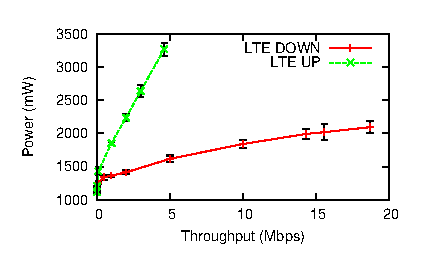
\includegraphics[width=.99\textwidth]{figures/mobisys12/power_tp.eps}
\ncaption{\small Power-throughput curve for LTE network}
\label{fig:power.tp}
\end{minipage}
\begin{minipage}[b]{.49\textwidth}
\centering
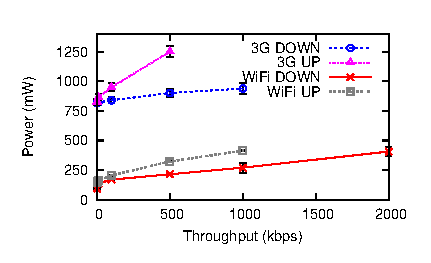
\includegraphics[width=.99\textwidth]{figures/mobisys12/power_tp2.eps}
\ncaption{\small Power-throughput curve for 3G and WiFi}
\label{fig:power.tp2}
\end{minipage}
\end{figure*}

\begin{figure}[t]
\centering
\IG{figures/mobisys12/up_down.eps} \\
\ncaption{Power of simultaneous uplink and downlink transfers}
\label{fig:up.down}
\end{figure}



\nsubsection{Power model for data transfer}
\label{sec:updown}
Previous work on 3G UMTS power modeling either treats DCH power state to have a fixed power value~\cite{codes.powertutor, mobisys.aro}, or assumes energy per bit to be the same constant for both uplink and downlink~\cite{imc.tailender}. These assumptions might be reasonable given that 3G has relatively low data rates. However, for LTE, we observe that device power is much higher during high speed data transmission (up to 3300mW for uplink) relative to the base power (1060mW) in \RC, and there is significant difference between downlink and uplink power levels at the same data rate. In this paper, we propose a new comprehensive power model for LTE empirically derived in a commercial LTE network.

We start with measuring device power states with controlled uplink or downlink throughput. The impact of TCP {\sf ACK} packets, which are small in size, is minor, thus ignored.

%TCP uplink data transfer incurs ACK packets in downlink direction, and vise versa. However, the impact of ACK packets is minor, which are smaller and fewer than data packets and the number of ACK packets.

Figures~\ref{fig:power.tp} and~\ref{fig:power.tp2} present the power-throughput curve for LTE, 3G, and WiFi. The curves are limited by the peak data rate we can achieve at the test location.
We observe that for all networks, a linear model fits well for both uplink and downlink. Assume uplink throughput is $t_u$ (Mbps) and downlink throughput is $t_d$ (Mbps), the power level (mW) for uplink is $P_u = \alpha_u t_u + \beta$ and for downlink $P_d = \alpha_d t_d + \beta$.
The best fit parameters are listed in Table~\ref{tab:up.down}.

\begin{table}[t]
\begin{center}
\begin{tabular}{|c|c|c|c|c|}\hline
 & $\alpha_u$ (mW/Mbps) & $\alpha_d$ (mW/Mbps) & $\beta$ (mW) & $\alpha_u/\alpha_d$ \\\hline
LTE & 438.39 & 51.97 & 1288.04 & 8.44\\\hline
3G & 868.98 & 122.12 & 817.88 & 7.12\\\hline
WiFi & 283.17 & 137.01 & 132.86 & 2.07\\\hline
\end{tabular}
\ncaption{Data transfer power model}
\label{tab:up.down}
\end{center}
\end{table}

By looking at $\alpha_u/\alpha_d$, we notice that uplink power increases faster than downlink for all three networks types. This is expected because sending data requires more power than receiving data for wireless data access~\cite{ieee.mimo}. LTE has the largest gap of $\alpha_u/\alpha_d = 8.44$ among three network types. This is largely because $\alpha_d$ for LTE is quite small. For 3G, both $\alpha_u$ and $\alpha_d$ are larger than LTE. $\beta$ is the base power when throughput is 0, with the ranking of LTE $>$ 3G $>$ WiFi. This is consistent with the tail base power comparison in Table~\ref{tab:power}. We notice that $\beta$ is slightly higher than the tail base for all networks types. This is possibly because of the overhead of switching transmitters or receivers into high speed mode.



For simultaneous uplink and downlink transfers, given that transmitters and receivers are separate, we conjecture that the power level (mW) is given by the following formula:
\begin{equation*}
P = \alpha_u t_u + \alpha_d t_d+ \beta
\end{equation*}
To validate this conjecture, we measure the power levels for concurrent uplink and downlink transfers in Figure~\ref{fig:up.down}. Assume total throughput $t = t_u + t_d$ and the ratio of uplink throughput $\epsilon = t_u \big/ t$:
\begin{equation*}
P = \alpha_u t_u + \alpha_d t_d+ \beta = (\alpha_u - \alpha_d)t\epsilon + \alpha_d t + \beta
\end{equation*}
When $t$ is a constant, $P$ grows linearly with $\epsilon$ and the slope is $(\alpha_u - \alpha_d)t$. Figure~\ref{fig:up.down} shows two curves of $t = 1$Mbps and $t = 2$Mbps, both having a strong linear pattern and the slope is less than 5\% off the expected value.


\nsubsection{Energy efficiency for bulk data transfer}
\label{sec:power.bulk}

\begin{figure}[t]
\centering
\IG{figures/mobisys12/energy_size.eps} \\
\ncaption{Energy per bit for bulk data transfers}
\label{fig:energy.size}
\end{figure}

To compare the power efficiency of different networks in the wild, we use bulk data transfer experiments to measure energy per bit.
Perrucci \etal~\cite{vtc.survey} measure energy per bit for 3G and WiFi with a fixed bulk size. In addition to taking LTE into consideration, we vary the bulk size to cover more possible network usage scenarios. Figure~\ref{fig:energy.size} shows the measured energy per bit in $\mu J / bit$ ($10^{-6} Joule / bit$) with different bulk data size. All data is randomly generated so that there is no chance for caching. We do not include promotion or tail energy but instead focus on data transfer energy. Given that signal strength and peak data rate on wireless networks fluctuates, both affecting energy per bit, our measurement only serves as a sampled view for the energy efficiency of different networks.
%\comment{why cite this study only?  it's the closest to ours?}

First, energy per bit decreases as bulk data size increases, largely because with a small data size, throughput does not reach link capacity due to TCP slow start. We also observe that LTE's energy per bit in downlink is comparable with WiFi, although the absolute power level of LTE is much higher than WiFi. This is due to high downlink throughput for LTE at our test location, even compared with the WiFi network. Similarly, for LTE uplink, it drops from 10$\mu J / bit$ to less than 1$\mu J / bit$ as bulk data size increases. With bulk data size of 10MB, LTE consumes 1.62 times the energy of WiFi for downlink and 2.53 for uplink. With lowest throughput, 3G has the worst energy efficiency for large data transfer, \eg for downloading 10MB data, 3G requires 21.50 times the energy of LTE and 34.77 times the energy of WiFi, and for uplink, 7.97 times of LTE and 20.16 times of WiFi.

%3G and LTE require 34.77 and 1.62 times the energy of WiFi, respectively, and for uplink, 3G/WiFi ratio is 20.16 and LTE/WiFi ratio is 2.53.
%\comment{I thought these numbers are interesting and should be included in the intro: in particular, you should have small transfer (1 packet) vs. bulk transfer energy per bit comparision}

\nsubsection{Power model validation}
\label{sec:power.validation}

\begin{table}[h]
\begin{center}
\begin{tabular}{|c|c|c|c|c|}\hline
\MR{App} & Measured & Simulated & \MR{Error}  \\
&energy (J)\footnotemark[1] & energy (J)\footnotemark[1] &\\\hline
Website G\footnotemark[3] & 24.77 & 24.37 & -1.61\% (-2.06\%\footnotemark[2]) \\\hline
Website Y\footnotemark[3] & 31.84 & 30.08 & -5.53\% (-7.04\%) \\\hline
YouTube & 21.81 & 21.14 & -3.07\% (-4.17\%) \\\hline
NPR News & 24.65 & 24.37 & -1.12\% (-1.70\%) \\\hline
Market & 38.64 & 38.03 & -1.58\% (-3.03\%) \\\hline
\end{tabular}
\\
\begin{tabular}{l}
{$^1$Both measured and simulated energy include tail energy}\\
{$^2$This error is for simulated energy assuming $\alpha_u = \alpha_d = 0$}\\
{$^3$Refer to \S\ref{sec:method.app}\comment{update reference} for the definition of \WG and \WY}\\
\end{tabular}
\ncaption{LTE power model validation}
\label{tab:power.validation}
\end{center}
\end{table}

To validate the LTE power model and the trace-driven simulation (\S\ref{sec:method.sim}), we compare measured energy (measured from the LTE phone) with simulated energy for case study applications. Table~\ref{tab:power.validation} contains the sample application usage scenarios described in \S\ref{sec:method.app}. The error rate is consistently less than 6\%, with the largest error rate from \WY, which includes heavy JavaScript execution and HTML rendering. Since our power model focuses on radio power and ignores the impact of CPU, for \WY, the total energy usage is slightly underestimated. 
%As we observe, the impact of non-network components on total energy is minor, except for the excluded screen. 

The error rate is increased if the impact of downlink and uplink throughput is ignored, \ie assuming $\alpha_u = \alpha_d = 0$. However, the increase is not significant, at most 1.5\%. This is because for these web-based applications, network throughput is low due to small object size (\S\ref{sec:app.perf}\comment{update reference}). For other applications, such as video/audio streaming and file download, we expect to see a larger gap in error rate if the impact of downlink/uplink is ignored.

In this section, in addition to comparing energy per bit in bulk data transfer for different networks, we construct a new LTE power model and validate its accuracy, which is the basis for the following analysis.


\nsection{User Trace Based Tradeoff Analysis}

\nsubsection{trace-driven network/power simulation methodology (validation)}
\S3.3

\nsubsection{\S6.1, 6.2, 6.3}


\chapter{Related Work}
\label{chap:related}

In this chapter, we summarize related work in different categories.

\nsection{Network and Application Performance Characterization}

Netdiff system~\cite{Mahajan:NSDI2008:NetDiff} establishes a benchmark for comparing performance of different ISPs. In our research, we attempt to establish an equivalent benchmark for comparing network application performance on smartphones. Although there are some existing tools available for such comparison, \eg Speedtest.net~\cite{speedtestnet} and FCC's broadband test~\cite{fccspeedtest}, which measure the throughput and latency in 3G networks, \mobiperf covers a more comprehensive set of metrics, including DNS lookup, Ping to the first hop, TCP handshake, and HTTP request to landmark servers, \etc Existing studies have compared 3G and WiFi performance on smartphones~\cite{Gass:3GWiFi:PAM2010} and studied the influence of the packet size on the delay in 3G networks~\cite{Arlos:OneWay:PAM2010}. Tan \etal carried out a similar measurement study on multiple commercial 3G networks~\cite{wltan07}. However, their study is limited to one location (Hong Kong) and a few devices. Compared with their study, our work covers significantly more users from many different locations. Netalyzr~\cite{netalyzr} carries out network measurement for Internet users, not for smartphone users.

Our work is inspired by numerous network measurement studies~\cite{Chakravorty:WWAN:Mobicom2004, Zhuang:A3:Mobicom2006, Ionut:Serendipity:IMC09, Mahesh:Ephemera:IMC09}, \eg Trestian \etal characterize the relationship between users' application interests and mobility ~\cite{Ionut:Serendipity:IMC09}, Zhuang \etal investigate application-aware acceleration to improve application performance~\cite{Zhuang:A3:Mobicom2006}, and Liu \etal study the interaction between the wireless channels and applications~\cite{Liu:3GChannelAppl:Mobicom2008}. Unlike these studies, we analyze the network performance along diverse dimensions, including continents, geographic locations, carriers, platforms, cellular technology, and time, \etc

In our previous work~\cite{sigmetrics.cluster}, we made qualitative observations on the effectiveness of CDN service in cellular networks and the geographical coverage of LDNS servers. In this study, with a comprehensive end-to-end latency measurement data set, we quantify the effectiveness of adopting different CDN servers for cellular networks. We also provide fine-grained analysis of the geographical coverage of each individual IP address of LDNS servers and discuss the implication on performance and reliability.

Existing work has built tools to infer traffic differentiation policies from either local experiments or public deployment~\cite{imc.netpolice, nsdi.glasnost, windrider}. And our work is among the first attempts to systematically uncover the previously unknown network policy in cellular networks.

There have been several studies focusing on mobile users from the perspective of applications, such as a study~\cite{Ionut:Serendipity:IMC09} which characterizes the relationship between users' application interests and mobility, and another study~\cite{Mahesh:Ephemera:IMC09} which examines the possibility of geolocating IP address in 3G networks. Other related measurement works of cellular data networks include a study of traffic characteristics on mobile devices~\cite{Maier:Traffic:PAM2010}, a performance study of multimedia streaming~\cite{Chesterfield:3GMultimedia:Monet2004}, and performance analysis of TCP/IP over 3G network with rate and delay variation~\cite{Mun:TCP/IP:Mobicom2002}. Our work complements these works with different focus and methodology. 

Unlike previous studies, \eg~\cite{Liu:3GChannelAppl:Mobicom2008, Chakravorty:WWAN:Mobicom2004, Jang:3G:MICNET2009}, which perform measurements on desktop or laptop systems, relying on cellular network data cards or phones tethered through USB as a modem, in this study, the data is collected directly from end-users' devices, thus more accurately reflecting the user-perceived performance.



+ on power footprint characterization

+ on application performance study

+ on mobile traffic pattern study

+ on TCP

+ on radio optimization


\nsection{Traffic}

We summarize three categories of work in understanding smartphones and mobile networks. %We summarize them in three categories.

\textbf{Characterizing Mobile Network Usage and Performance.}
Prior efforts~\cite{falaki10_mobisys, shepard10, qian13_pam} deployed smartphone user studies and collected data from tens to hundreds of participating users. Those studies investigated various aspects including the diversity of smartphone users, the popularity of mobile applications, and the effectiveness of compression techniques on cellular traffic \etc. The 3G Test study~\cite{mobisys.3gtest} adopts another approach by publishing an app that actively measures various network performance metrics on users' handsets. Our study features a much larger user base of around 300K customers using the LTE networks whose characteristics are far from being well understood. Some previous studies also performed large-scale measurement of mobile networks and smartphones.
Sommers \etal compared cellular and Wi-Fi performance using crowd-sourced data from \texttt{speedtest.net} covering 15 metro areas, focusing on throughput and latency~\cite{sommers12}. Xu \etal profiled diverse usage behaviors of smartphone applications~\cite{xu11_imc}. Qian \etal performed network-wide measurement studies of cellular periodic transfers~\cite{qian12_www}. In contrast, our investigated spectrum is more diverse, covering
traffic characteristics, network performance, protocol interaction, bandwidth utilization, and application usage in the increasingly popular LTE networks. We also compare our results with those presented in~\cite{mobisys.3gtest} and~\cite{sommers12}. Some previous studies~\cite{gember11, chen12} also examined mobile handsets using Wi-Fi networks.

\textbf{Cellular Resource Management and Cross-layer Interaction.} In cellular networks, there exists a radio resource control (RRC) state machine that manages the handset radio interface. It is the key coupling factor bridging the application traffic patterns and the lower-layer protocol behaviors. Previous studies~\cite{imc.3g} and~\cite{huang12_mobisys} examine the RRC state machine and its interaction with cellular traffic, for 3G UMTS and 4G LTE networks, respectively. We study for hundreds of thousands of users their state transition delay and transport-layer idle time, two key factors incurring signaling load and energy overhead, respectively, due to the LTE RRC state machine.
Previous studies also examined the interplay between TCP and cellular networks. For example, Liu \etal studied the physical and MAC layers in 3G EvDO networks and their impact on TCP performance~\cite{Liu:3GChannelAppl:Mobicom2008}. Jiang \etal examined how large buffers in cellular networks contribute to significant TCP queuing delay~\cite{jiang12}. Our study brings new insight into the complex interaction between LTE and TCP, as detailed in~\S\ref{sec:char}.

\textbf{Cellular Network Infrastructure.}
%Using a data-driven approach, 
Xu \etal characterized 3G data network infrastructures, leading to an observation that the routing of cellular data traffic is quite restricted as traffic must traverse through a small number of gateway nodes~\cite{sigmetrics.cluster}. %Yellowpage
Wang \etal unveiled cellular carriers' NAT and firewall policies~\cite{sigcomm.nat}. %NetPiculet
Balakrishnan \etal investigated IP address dynamics in 3G networks. They found that cellular IPs embed much less geographical
information than wired IPs do~\cite{Mahesh:Ephemera:IMC09}. %IMC 09 Where��s that Phone?
In this work, characterizing LTE infrastructures is not our immediate focus, but we do have novel findings that they highly affect our measurement methodology and results as pinpointed in~\S\ref{sec:char} and~\S\ref{sec:estimate}.


\nsection{Mobisys12}

We summarize related work in three categories below.

\textbf{Measuring 2G and 3G networks.} Prior study~\cite{imc.tailender} investigates the impact and the optimization of tail effects in 2G/3G networks. Previous work~\cite{imc.3g} characterizes the impact of RRC state machine on radio resources and energy by analyzing a dataset collected from a commercial UMTS network. Recent work~\cite{falaki10_imc} also investigates impact of traffic patterns on radio power management policy. Other measurement studies (\eg 3GTest~\cite{mobisys.3gtest}, LiveLab~\cite{shepard10}, and~\cite{falaki10_mobisys}) collect traces from real smartphone users, focusing on characterization at only IP and higher layers. None of them investigate resource management policy in 4G LTE networks.

\textbf{Smartphone power modeling} has also been investigated by previous empirical measurements. The Bartendr project~\cite{mobicom.bartendr} studies the relationship between signal strength and smartphone radio power usage. PowerTutor~\cite{codes.powertutor} collects power traces for individual hardware components under controlled experiments then uses multi-variable regression to compute the coefficients for a linear power model considering all hardware components. ARO~\cite{mobisys.aro} employs an approach similar to~\cite{codes.powertutor} but focusing only on radio power usage. It performs more fine-grained simulation of transmission queues to capture state transitions. Our LTE power model is also empirically derived, but it differs from all aforementioned models in two aspects. First, it considers DRX in \RC, a new power management mechanism in LTE networks. Second, it further takes into account both uplink and downlink data rates, resulting in a more accurate estimation of the radio power consumption when the throughput is high, as is a common case in LTE networks.

\textbf{DRX in 4G LTE networks.} Zhou \etal~\cite{vtc.drx} model the DRX mechanism as a semi-Markov process, with which they analytically study the effects of DRX parameters on the performance, as well as the tradeoff between the power saving and wake-up delay. Kolding \etal~\cite{iswcs.lte} also investigate the balance between throughput and power saving by changing the configuration of DRX parameters, using a web-browsing traffic model. Bontu \etal~\cite{ieee.drx} further considers the impact of DRX parameters on different applications with various delay sensitivities. Wigard \etal compares a long-DRX-only scenario and a scenario with both long and short DRX, in terms of throughput and power consumption. All above studies employing analytical models suffer from an inherent limitation: the expressiveness of an analytical model is quite limited and is unlikely to capture the characteristics of real-world traffic patterns using a statistical distribution with a few parameters. The existence of concurrent applications accessing the network further increases the difficulty of modeling the packet dynamics. In contrast, our work is the first empirical study to investigate the impact of the configurations of DRX parameters and tail timer. We overcome the above limitation by employing network traces from real smartphone users, thus more realistically revealing the complex tradeoffs incurred by various DRX parameters.

%Lin Zhong why browsers are slow~\cite{hotmobile.web} 


\nsection{Screen}
Smartphones with cellular data access have become increasingly popular across the globe, with the wide deployment of 3G and emerging LTE~\cite{3gpp.lte} networks, and a plethora of applications of all kinds. Cellular networks are typically characterized by limited radio resources and significant device power consumption for network communications. The battery capacity of smartphones cannot be easily improved due to physical constraints in size and weight. Hence, battery life remains a key determinant of end-user experience. Given the limited radio resources in these networks and device battery capacity constraints, optimizing the usage of these resources is critical for cellular carriers and application developers.
%, leading many consumers to treat battery life as an important criterion for choosing devices.

In 3G and 4G cellular networks, the user equipment (UE) must stay in a high-power state, occupying radio resources for some required time before the allocated resource is released by the network, and then the UE enters a low power state. This required time period, also known as the Radio Resource Control (RRC) tail~\cite{imc.tailender}, is necessary and important for cellular networks to prevent frequent state promotions (resource allocation), which can cause unacceptably long delays for the UE, as well as additional processing overheads for the radio access network~\cite{poor, infocom_lee}. Today's cellular carriers use a static and conservative setting of the tail time in the order of many seconds, and previous studies have revealed this tail time to be the root cause of energy and radio resource inefficiencies in both 3G~\cite{imc.3g, imc.tailender, wts04, Chuah:Impacts:WCNC2002} and 4G networks~\cite{huang12_mobisys}. Various optimization solutions have been proposed to address this problem, \eg the use of fast dormancy~\cite{fast.dormancy.1, fast.dormancy.2, qian10_icnp} and client-side traffic shaping and scheduling~\cite{qian12_www, mobisys10_ra, imc.tailender}. In addition, specialized energy saving techniques for mobile applications have been proposed for specific applications~\cite{mobisys09_wang, mobisys08_kang} and for specific protocols~\cite{mobisys07_agarwal}.


{\em  Fast dormancy (FD)}~\cite{fast.dormancy.1, fast.dormancy.2} is a mechanism in 3G networks for reducing the amount of tail time incurred by a device by quickly demoting it to a low energy RRC state without waiting for the tail timer to expire.




\nsection{RadioProphet}

%\textbf{Radio resource management} has become a critical topic given the explosive growth of cellular data traffic.

We describe related work in four categories below.

\textbf{Investigation of the inactivity timers in cellular networks.} Inactivity timers, which determine the tail times, are the most important parameters in cellular radio resource management. Previous works study the impact of inactivity timers on the UMTS network capacity~\cite{Chuah:Impacts:WCNC2002} and the UE energy consumption~\cite{Lee:Impact:WTS2004, Yeh:Energy:ITVT2009}.
%by simulating the performance of web browsing.
%propose analytical models to measure the energy consumption of user device under different timer values.
Another study~\cite{imc.3g} makes a further step by characterizing the impact of operational state machine settings with real traces and conclude that the fundamental limitation of the current cellular resource management mechanism is treating all traffic according to the same RRC state machine \emph{statically and globally} configured for all users, therefore, it is difficult to balance various tradeoffs of resource utilization.

\textbf{Adaptive resource release.}
Distinct from using static timers, Liers~\etal~\cite{Liers:DynamicTimeout:PIMRC2005} propose to determine inactivity timers dynamically. %based on the current load, radio resources, and processing capability.
However, they only address the problem from the perspective of network capacity as to reducing the call blocking and dropping rate, and the same timer values are applied globally to all UEs at any given time. In comparison, \NAME is based on fast dormancy where resource release is requested by each individual UE. Such fine-grained control leads to much more significant savings of the radio resource and the UE energy consumption.

%The key challenge addressed by TOP is to handle  network activities of concurrently running applications.

TOP~\cite{qian10_icnp} proposes to leverage fast dormancy to eliminate the tail whenever possible. It {\em \bf assumes} each individual application can predict an imminent long \IBT with reasonable accuracy, and fast dormancy is only invoked when the predicted aggregate idle time across all concurrent applications is long enough. While TOP provides framework and mechanism for optimization, it does {\em not} solve the problem of prediction. In this study, we solve the open research problem of predicting \IBTS. Unlike TOP being a proposed framework with unsolved assumptions, our system \NAME is a practical working system.

MakeIdle~\cite{makeidle} uses packet timestamp information to calculate the optimal idle time before fast dormancy should be invoked that maximizes the energy saving. However, MakeIdle does not look at the application context and other useful features used in \NAME, resulting in worse performance as shown later. Moreover, MakeIdle algorithm does not consider the balance of energy saving and signaling overhead, and leaves the job of reducing the signaling overhead to another algorithm called MakeActive~\cite{makeidle}, based on shifting packets (batching). MakeActive does not work for foreground traffic, and even for background traffic, there is no guarantee that it would not affect user experience, since it may incur up to seconds extra delay. In this study, to minimize such negative impact on user experience, \NAME does not rely on any traffic shifting techniques, especially because the goal for the design of \NAME is to be working for all traffic, both foreground and background.

RadioJockey\cite{radiojockey} is another closely related study. It uses system call traces to determine the {\em end-of-session} (EOS) for each application and triggers fast dormancy if there is no active session for any of the applications. However, RadioJockey only works for background application with no user interaction, and the authors point out that the prediction accuracy would be lower for foreground traffic since user interactions may violate the correlation between system call patterns and EOS; while for \NAME, there is no such limitation and we achieve even better performance for all traffic than RadioJockey for screen-off traffic. Also, RadioJockey treats different applications separately and could not predict the {\em start-of-session} (SOS), hence when there are multiple concurrent applications, the prediction accuracy would be jeopardized, with higher instrumentation and prediction overhead. Our approach uses aggregate traffic from all applications and does not suffer from these problems. Further, RadioJockey requires complete system call traces for all applications in addition to the network traces, which incurs higher overhead than \NAME. In the evaluation section later, we compare both MakeIdle and RadioJockey with \NAME and ignore MakeActive because it alters user traffic resulting in negative impact on user experience, which is not acceptable especially for foreground traffic.


\textbf{Traffic scheduling} There exists various traffic scheduling algorithms (\eg piggyback, batching~\cite{qian12_www}, TailEnder~\cite{imc.tailender}, and Intentional Networking~\cite{higgins10}) for optimizing resource consumption in cellular networks. For example, in piggyback~\cite{qian12_www}, transfers can be shifted earlier, or be postponed till later, so that they can potentially be overlapped with non-target transfers, thus reducing the total tail time. TailEnder~\cite{imc.tailender} schedules transfers to minimize the energy consumption while meeting user-specified deadlines by delaying transfers and transmitting them together. The major limitations of these approaches is that they are only applicable to delay-tolerant traffic (RSS feeds, push notification \etc). \NAME can be applied to any type of traffic (in particular, delay-sensitive traffic triggered by users), and can be used together with the aforementioned scheduling techniques.

\textbf{Traffic modeling and prediction} has be explored by various previous works. A linear prediction-based time series forecasting technique is used to predict future no-data intervals for multimedia data streaming~\cite{wcnc04}. Hidden Markov Models are also used for modeling and predicting traffic of several Internet applications~\cite{Dainotti20082645}. In our work, we look at the aggregate traffic, including all different applications, and predict whether inter burst time is longer than a threshold, which is a joint effect of packets generated by all applications, and hence is more challenging and better for practical use. This specific, yet important problem for energy and network resource saving has not been studied before in mobile platforms with a large real-world data set as ours.

\chapter{Conclusion and Future Work} \label{chap:conc}
aa

\section{Future Work}
blabla


\startappendices
  \appendix{List of top domain names for DNS loopup test}

The following list of top 100 domain names was obtained from Alexa~\cite{alexa} in 2009.

\lstset{language=C++}
\begin{lstlisting}
// List of top domain names for DNS lookup test in C++
char* DOMAIN_NAMES[] = {"yahoo.com", "google.com", "youtube.com", "live.com", "facebook.com", "msn.com", "myspace.com", "wikipedia.org", "blogger.com", "yahoo.co.jp", "baidu.com", "rapidshare.com", "microsoft.com", "google.co.in", "google.de", "hi5.com", "qq.com", "ebay.com", "google.fr", "sina.com.cn", "google.co.uk", "mail.ru", "orkut.com.br", "fc2.com", "aol.com", "vkontakte.ru", "google.com.br", "wordpress.com", "google.it", "flickr.com", "photobucket.com", "yandex.ru", "google.es", "google.co.jp", "google.cn", "amazon.com", "go.com", "naver.com", "craigslist.org", "friendster.com", "odnoklassniki.ru", "orkut.co.in", "google.com.mx", "imdb.com", "bbc.co.uk", "youporn.com", "taobao.com", "cnn.com", "adultfriendfinder.com", "googlesyndication.com", "skyrock.com", "163.com", "redtube.com", "imageshack.us", "youku.com", "ask.com", "google.ca", "uol.com.br", "pornhub.com", "espn.go.com", "adobe.com", "rakuten.co.jp", "orkut.com", "sohu.com", "ebay.de", "netlog.com", "apple.com", "dailymotion.com", "mixi.jp", "metroflog.com", "rambler.ru", "daum.net", "vmn.net", "rediff.com", "livedoor.com", "yahoo.com.cn", "google.com.tr", "fastclick.com", "fotolog.net", "livejournal.com", "about.com", "megavideo.com", "nytimes.com", "globo.com", "nicovideo.jp", "wretch.cc", "mininova.org", "soso.com", "google.com.au", "ameblo.jp", "nasza-klasa.pl", "google.pl", "goo.ne.jp", "google.co.id", "google.com.sa", "ku6.com", "yourfilehost.com", "imagevenue.com", "bebo.com", "comcast.net"};
\end{lstlisting}


\begin{singlespace}
\bibliographystyle{aiaa}
\bibliography{./thesis}
\end{singlespace}

\end{document}
